% ============================================================
% latex_includes.tex — 华中杯 B题：反射的艺术
% 使用方法：在主文档中 % ============================================================
% latex_includes.tex — 华中杯 B题：反射的艺术
% 使用方法：在主文档中 % ============================================================
% latex_includes.tex — 华中杯 B题：反射的艺术
% 使用方法：在主文档中 % ============================================================
% latex_includes.tex — 华中杯 B题：反射的艺术
% 使用方法：在主文档中 \input{figures/latex_includes.tex}
% 需要：\usepackage{float,booktabs,graphicx,subfig}
% ============================================================

% ============================================================
% 问题一：圆柱镜反射逆映射模型
% ============================================================

% --- 坐标系与三维几何关系 ---
\begin{figure}[H]
\centering
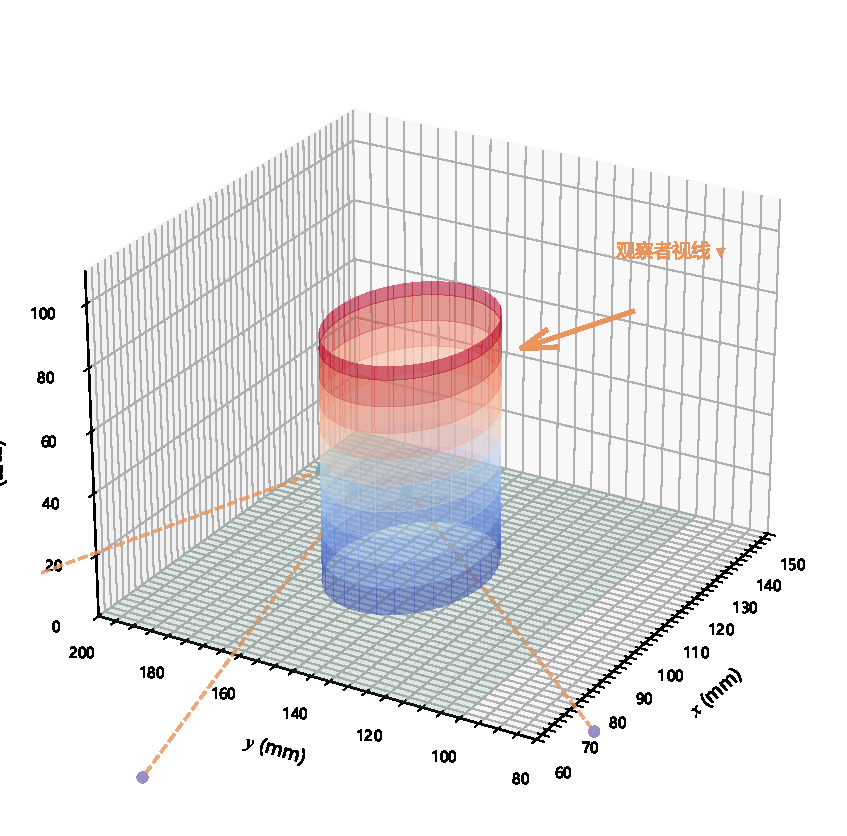
\includegraphics[width=0.72\textwidth]{figures/fig_coordinate_system.pdf}
\caption{圆柱镜反射坐标系示意图：展示纸面、圆柱镜、观察者视线及反射光路的三维空间关系}\label{fig:coordinate_system}
\end{figure}

% --- 逆映射畸变分布热力图 ---
\begin{figure}[H]
\centering
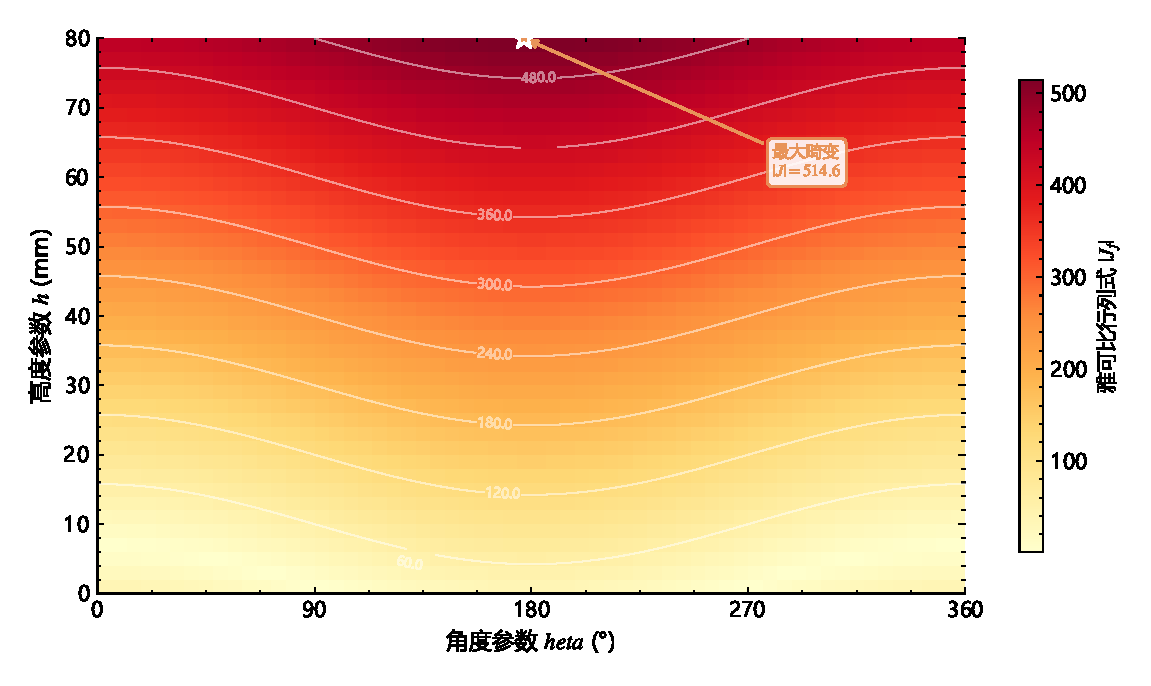
\includegraphics[width=0.72\textwidth]{figures/fig_mapping_distortion.pdf}
\caption{逆映射雅可比行列式在纸面上的分布热力图：颜色越深表示局部畸变越大}\label{fig:mapping_distortion}
\end{figure}

% --- 蒙娜丽莎四步闭环验证 ---
\begin{figure}[H]
\centering
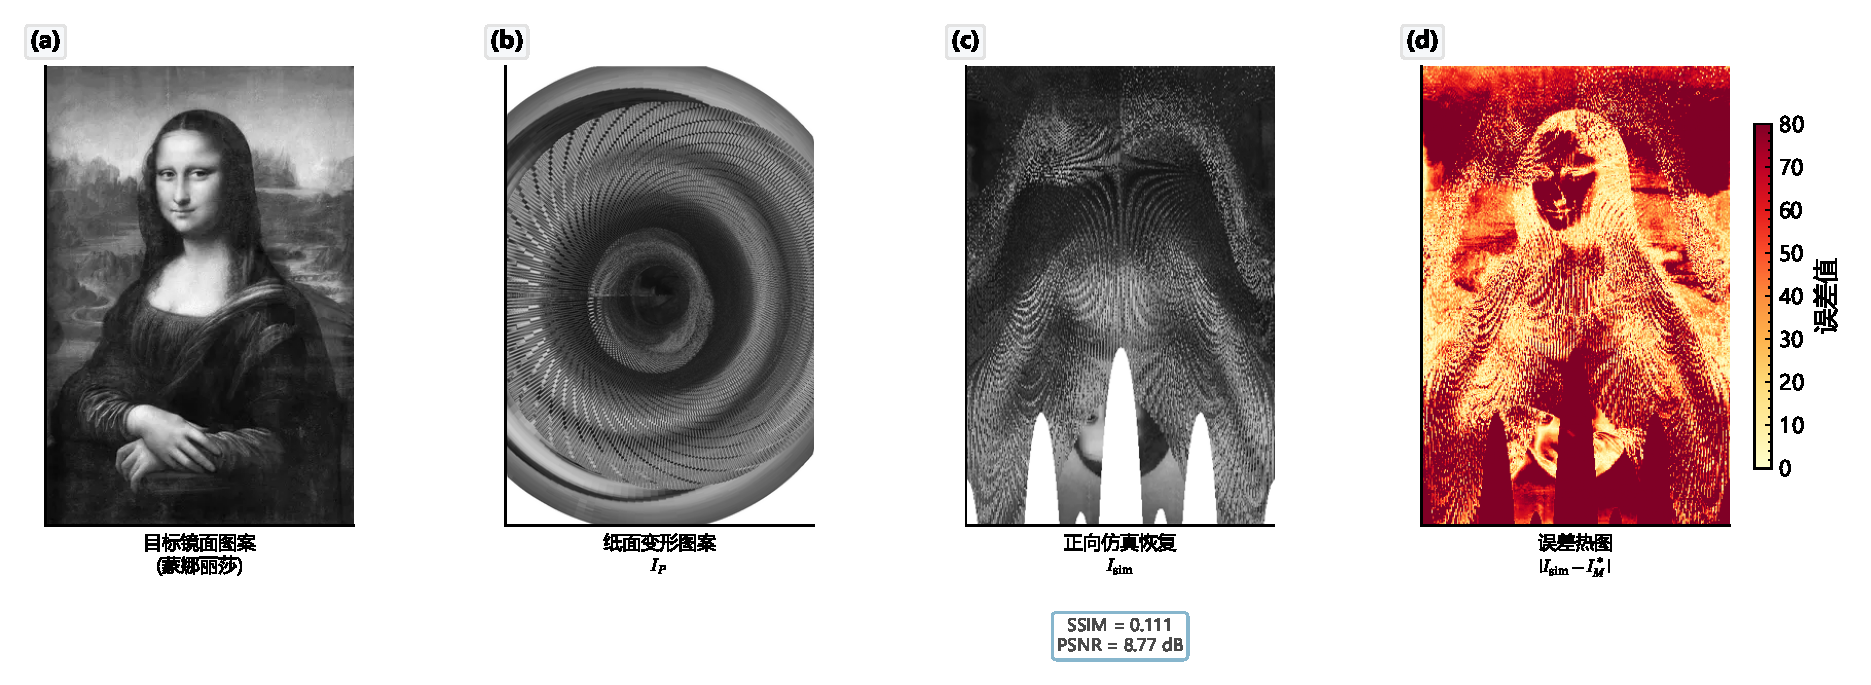
\includegraphics[width=0.95\textwidth]{figures/fig_monalisa_result.pdf}
\caption{图3（蒙娜丽莎）设计方案：目标镜面图案、生成纸面图案、正向仿真恢复图及误差热图}\label{fig:monalisa_result}
\end{figure}

% --- 卡通猫四步闭环验证 ---
\begin{figure}[H]
\centering
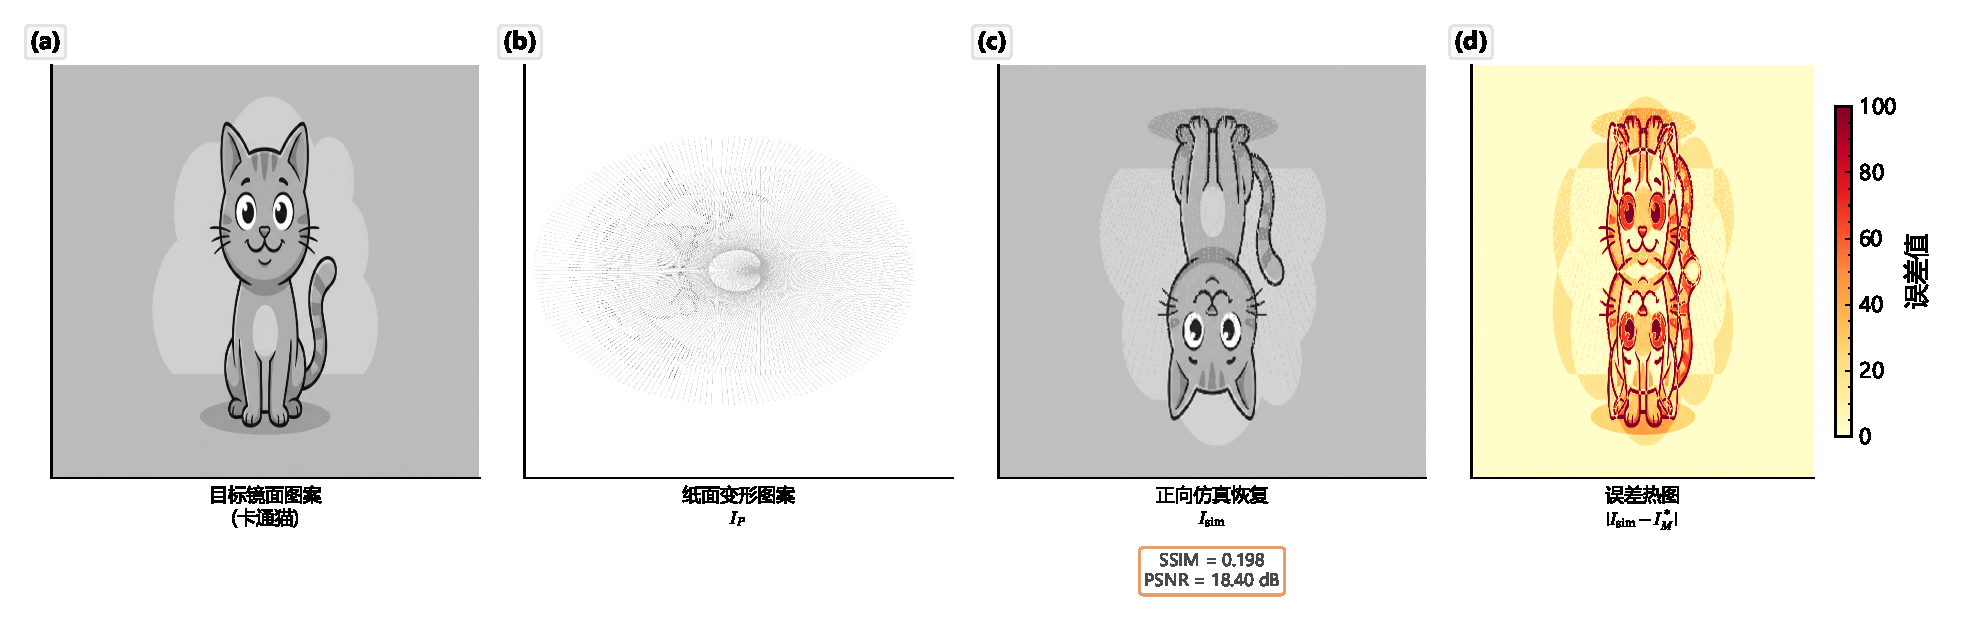
\includegraphics[width=0.95\textwidth]{figures/fig_cat_result.pdf}
\caption{图4（卡通猫）设计方案：目标镜面图案、生成纸面图案、正向仿真恢复图及误差热图}\label{fig:cat_result}
\end{figure}

% --- 最优圆柱参数对比表 ---
\input{figures/TABLE_param_optimal.tex}

% --- 图像质量评价指标对比表 ---
\input{figures/TABLE_image_metrics.tex}

% --- 双参数灵敏度等高线（R 与位置偏移对 SSIM 的影响）---
\begin{figure}[H]
\centering
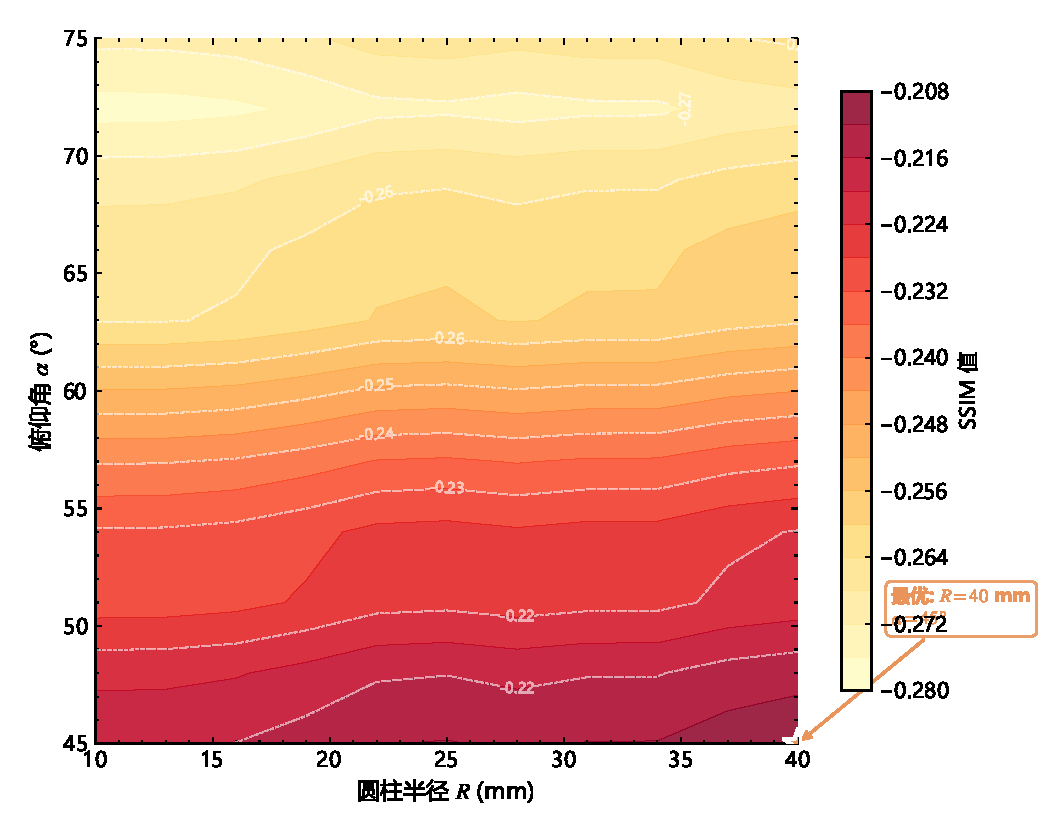
\includegraphics[width=0.72\textwidth]{figures/fig_param_optimization.pdf}
\caption{圆柱半径 $R$ 与位置偏移对 SSIM 的双参数灵敏度等高线图：星号标注最优参数组合}\label{fig:param_optimization}
\end{figure}

% --- 不同参数组合下 SSIM/PSNR 分组柱状图 ---
\begin{figure}[H]
\centering
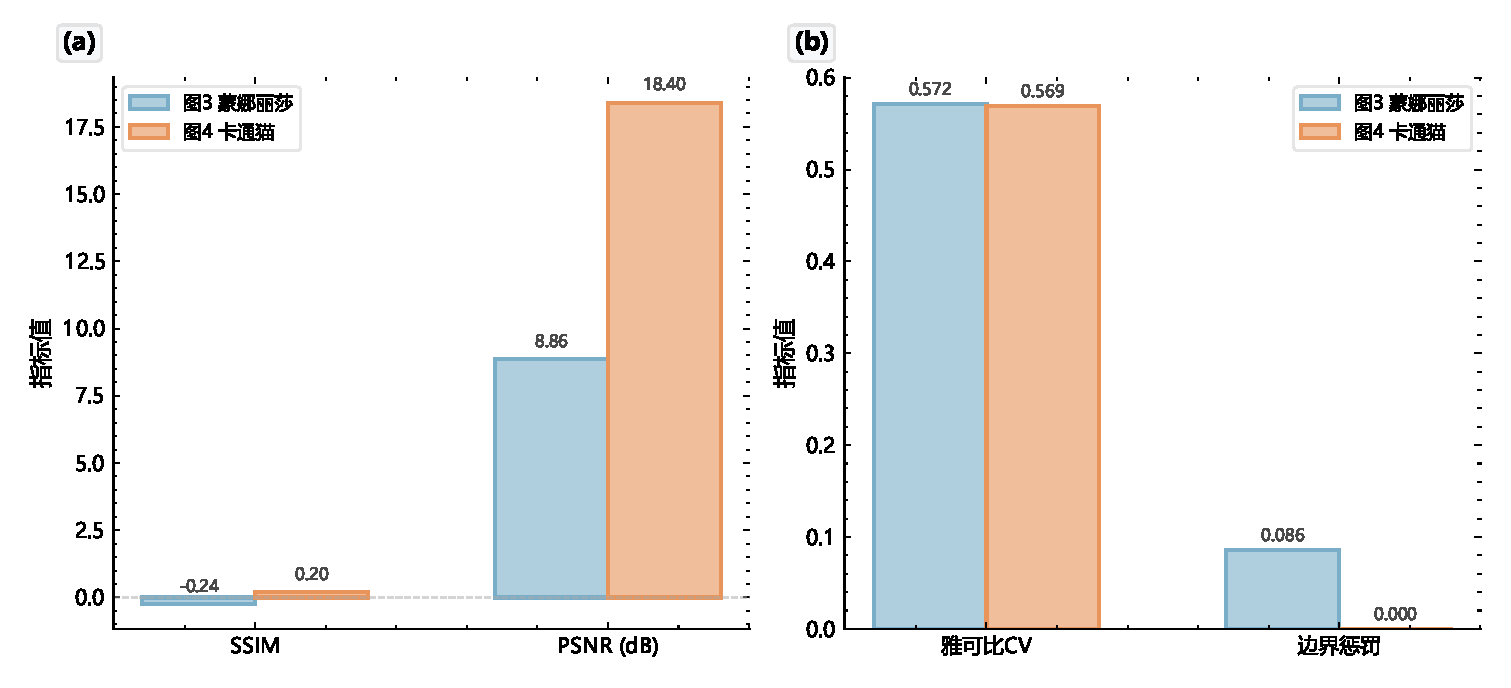
\includegraphics[width=0.80\textwidth]{figures/fig_ssim_comparison.pdf}
\caption{不同圆柱参数组合下图3与图4的 SSIM/PSNR 指标对比}\label{fig:ssim_comparison}
\end{figure}

% ============================================================
% 问题二：纸面与镜面图案双有意义设计
% ============================================================

% --- 双有意义案例展示 ---
\begin{figure}[H]
\centering
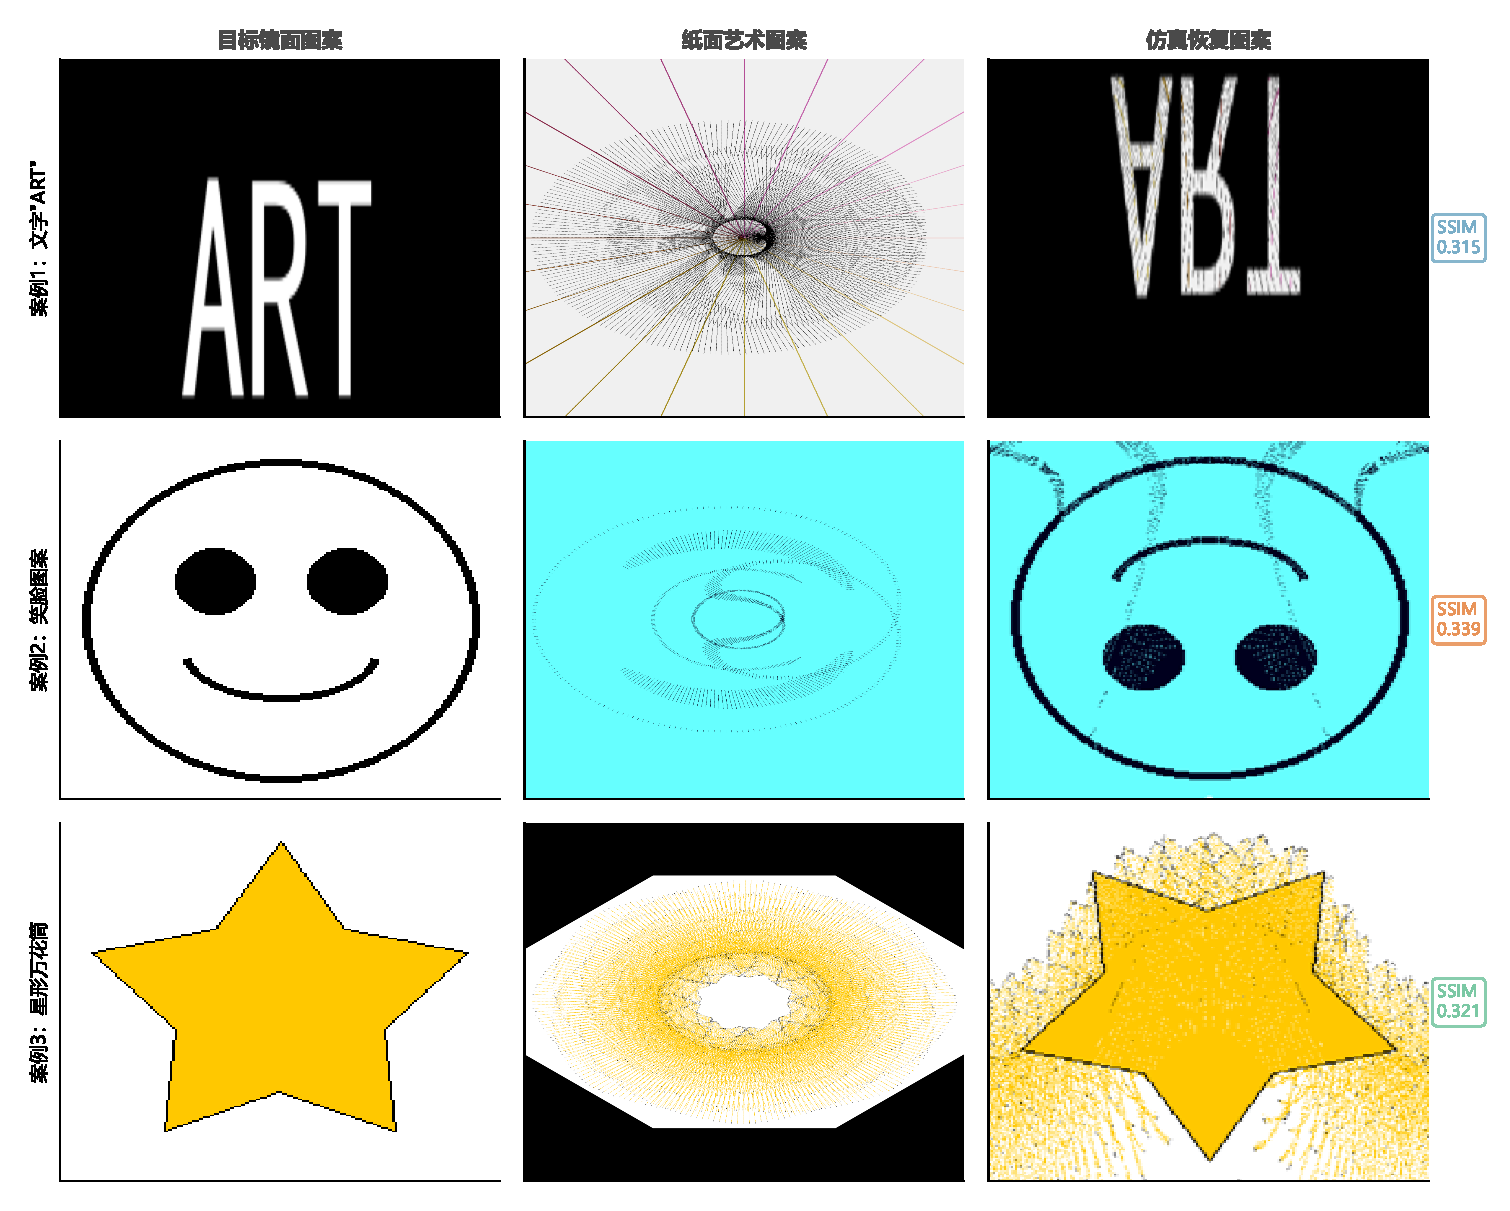
\includegraphics[width=0.95\textwidth]{figures/fig_dual_meaning_cases.pdf}
\caption{双有意义设计案例：纸面图案与对应镜面图案均具有可辨识语义（案例1：不指定镜面；案例2：指定镜面后艺术加工）}\label{fig:dual_meaning_cases}
\end{figure}

% --- 频谱特征与镜面可辨识度关系 ---
\begin{figure}[H]
\centering
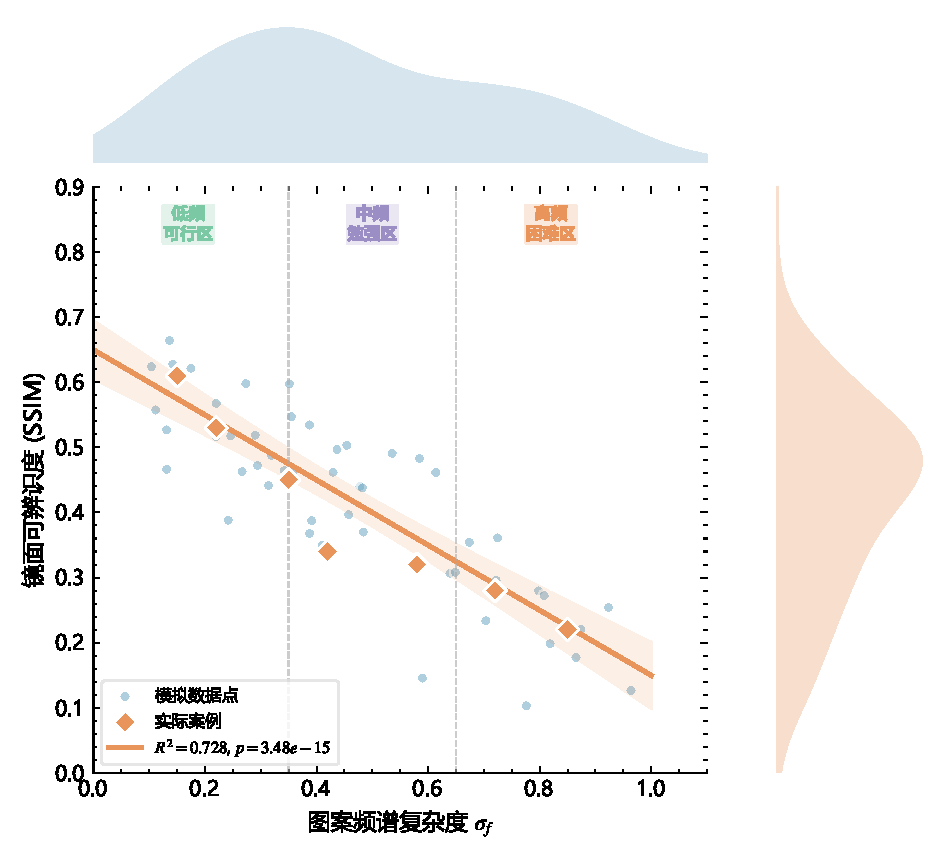
\includegraphics[width=0.72\textwidth]{figures/fig_frequency_analysis.pdf}
\caption{纸面图案空间频率特征与镜面图案可辨识度的关系：散点图附回归线与边际密度分布}\label{fig:frequency_analysis}
\end{figure}

% ============================================================
% 问题三：双目标兼容性理论模型
% ============================================================

% --- 兼容性相图 ---
\begin{figure}[H]
\centering
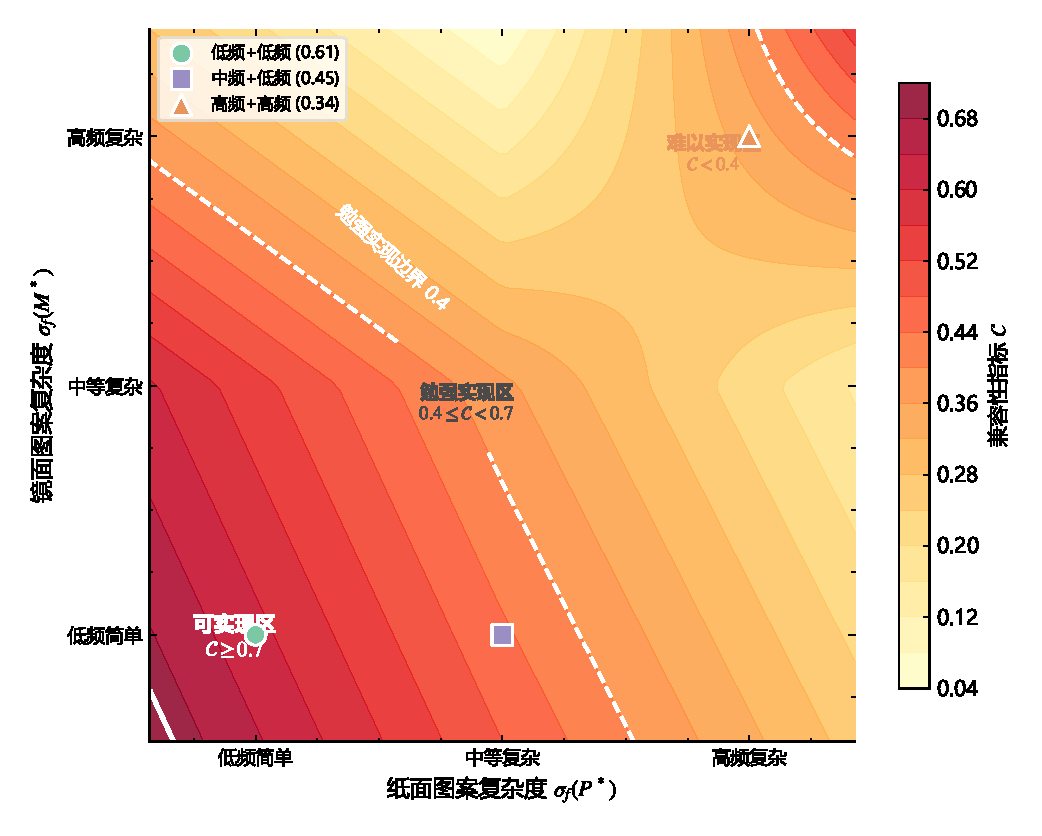
\includegraphics[width=0.72\textwidth]{figures/fig_compatibility_phase.pdf}
\caption{纸面-镜面图案兼容性相图：以纸面复杂度与镜面复杂度为坐标轴，划分可实现区、勉强实现区与难以实现区}\label{fig:compatibility_phase}
\end{figure}

% --- Pareto 前沿图 ---
\begin{figure}[H]
\centering
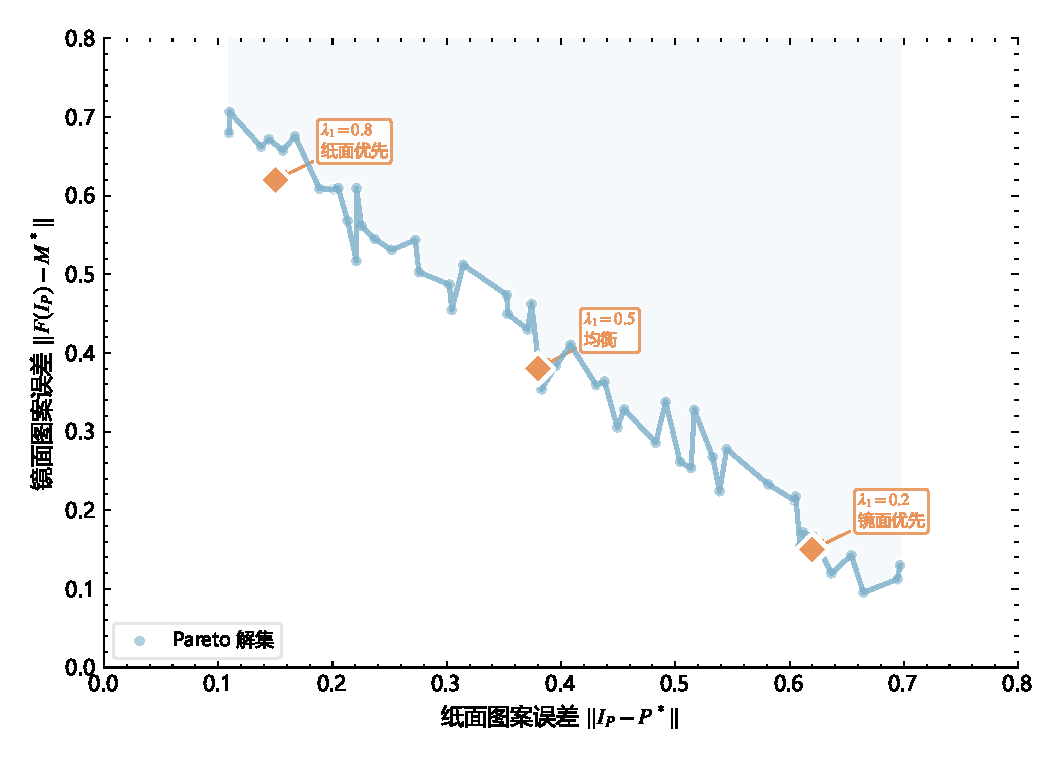
\includegraphics[width=0.68\textwidth]{figures/fig_dual_objective_pareto.pdf}
\caption{双目标优化 Pareto 前沿：纸面误差与镜面误差之间的权衡关系}\label{fig:dual_objective_pareto}
\end{figure}

% --- 多维兼容性雷达图 ---
\begin{figure}[H]
\centering
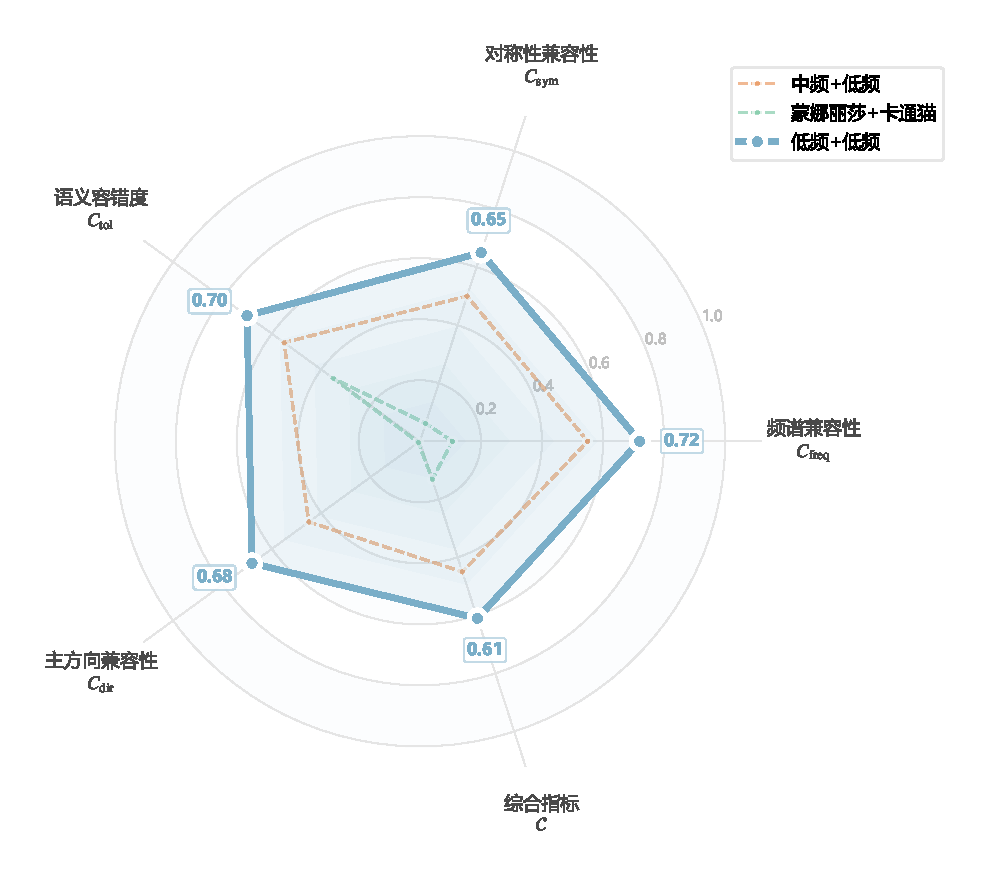
\includegraphics[width=0.65\textwidth]{figures/fig_compatibility_radar.pdf}
\caption{不同图案组合在频谱兼容性、对称性兼容性、语义容错度等多维指标上的雷达图对比}\label{fig:compatibility_radar}
\end{figure}

% --- 兼容性评分汇总表 ---
\input{figures/TABLE_compatibility.tex}

% ============================================================
% 灵敏度分析
% ============================================================

% --- 圆柱半径 R 对 SSIM 的影响折线图 ---
\begin{figure}[H]
\centering
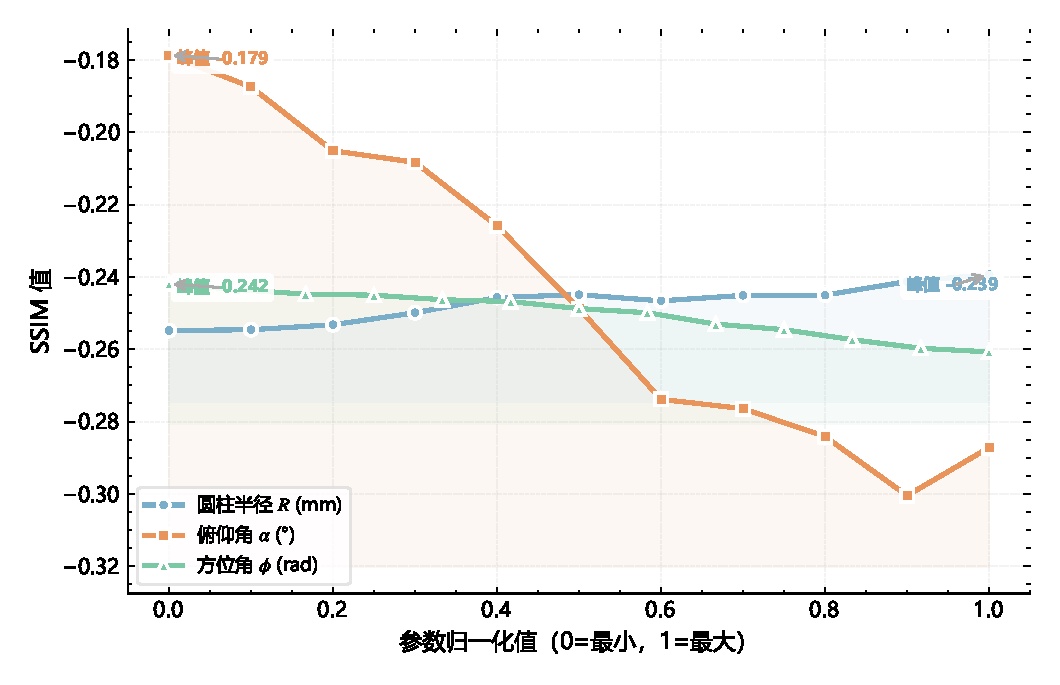
\includegraphics[width=0.72\textwidth]{figures/fig_sensitivity_R.pdf}
\caption{圆柱半径 $R$ 变化对 SSIM 的影响曲线（含 95\% 置信区间）}\label{fig:sensitivity_R}
\end{figure}

% --- 多参数灵敏度汇总热力图 ---
\begin{figure}[H]
\centering
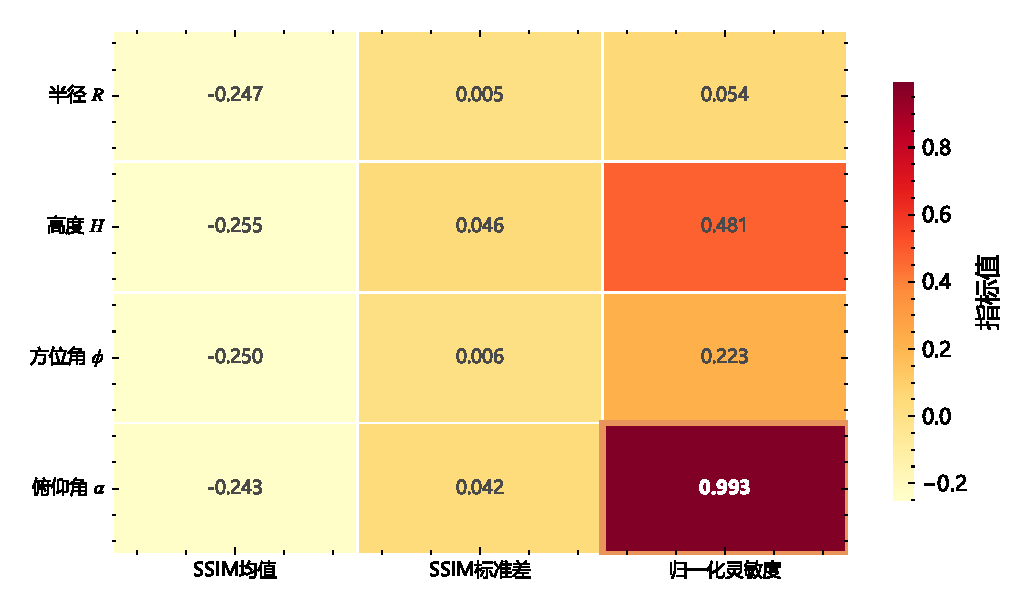
\includegraphics[width=0.72\textwidth]{figures/fig_sensitivity_heatmap.pdf}
\caption{多参数灵敏度汇总热力图：$R$、$H$、$\phi$、$\alpha$ 对 SSIM、PSNR 及雅可比 CV 的影响程度}\label{fig:sensitivity_heatmap}
\end{figure}

% --- 灵敏度分析汇总表 ---
\input{figures/TABLE_sensitivity.tex}

% 需要：\usepackage{float,booktabs,graphicx,subfig}
% ============================================================

% ============================================================
% 问题一：圆柱镜反射逆映射模型
% ============================================================

% --- 坐标系与三维几何关系 ---
\begin{figure}[H]
\centering
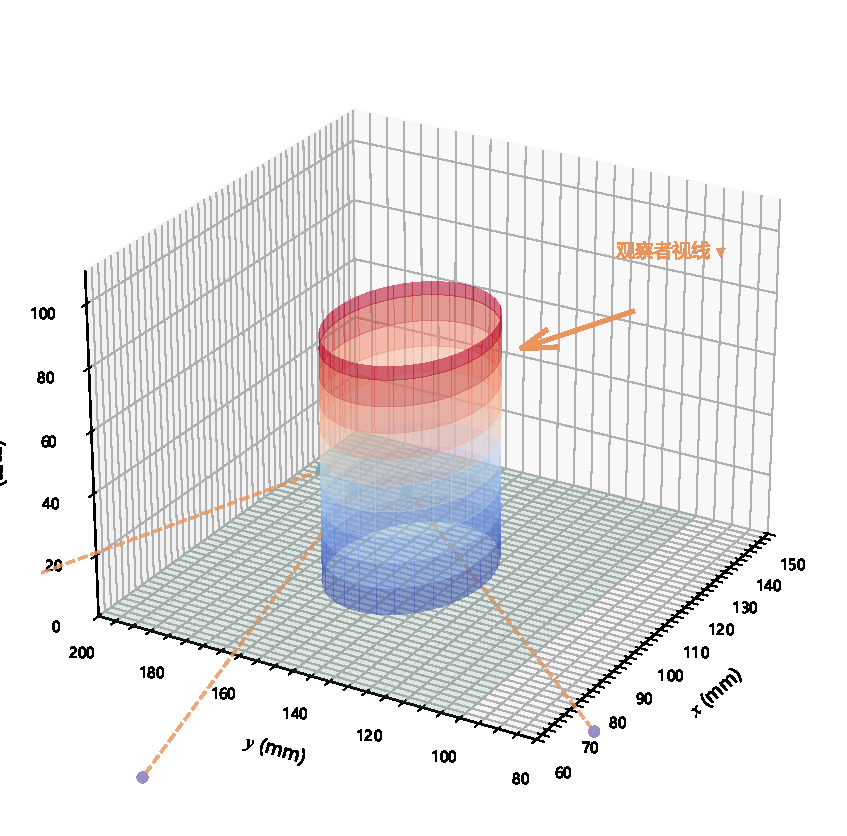
\includegraphics[width=0.72\textwidth]{figures/fig_coordinate_system.pdf}
\caption{圆柱镜反射坐标系示意图：展示纸面、圆柱镜、观察者视线及反射光路的三维空间关系}\label{fig:coordinate_system}
\end{figure}

% --- 逆映射畸变分布热力图 ---
\begin{figure}[H]
\centering
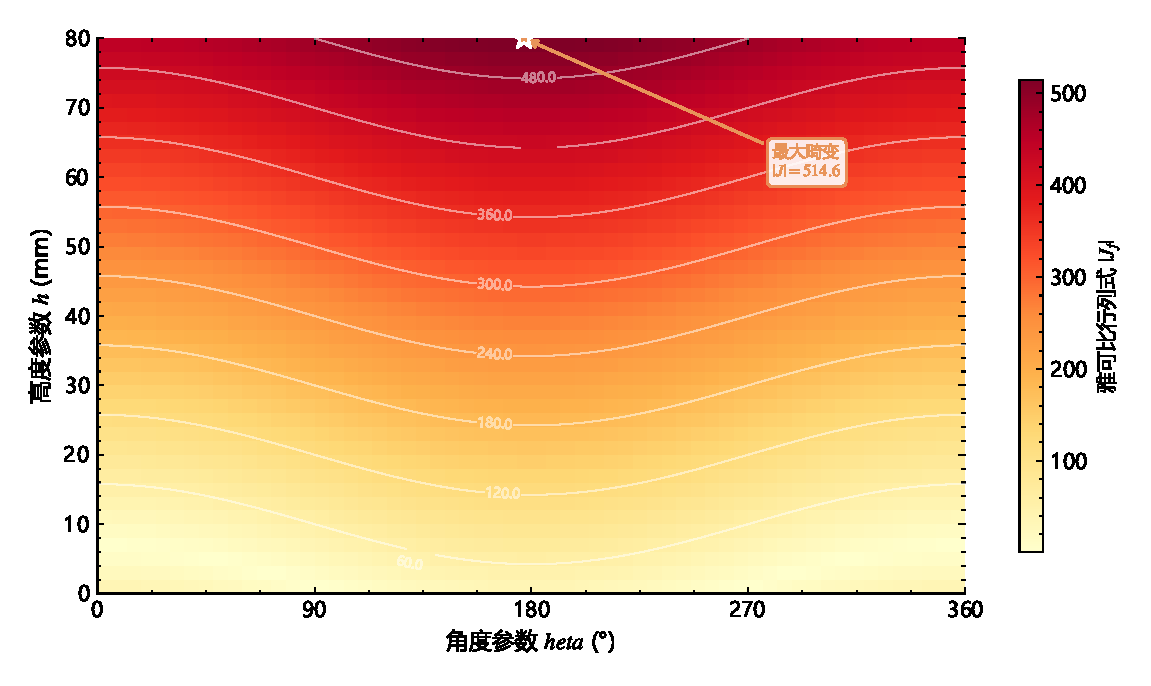
\includegraphics[width=0.72\textwidth]{figures/fig_mapping_distortion.pdf}
\caption{逆映射雅可比行列式在纸面上的分布热力图：颜色越深表示局部畸变越大}\label{fig:mapping_distortion}
\end{figure}

% --- 蒙娜丽莎四步闭环验证 ---
\begin{figure}[H]
\centering
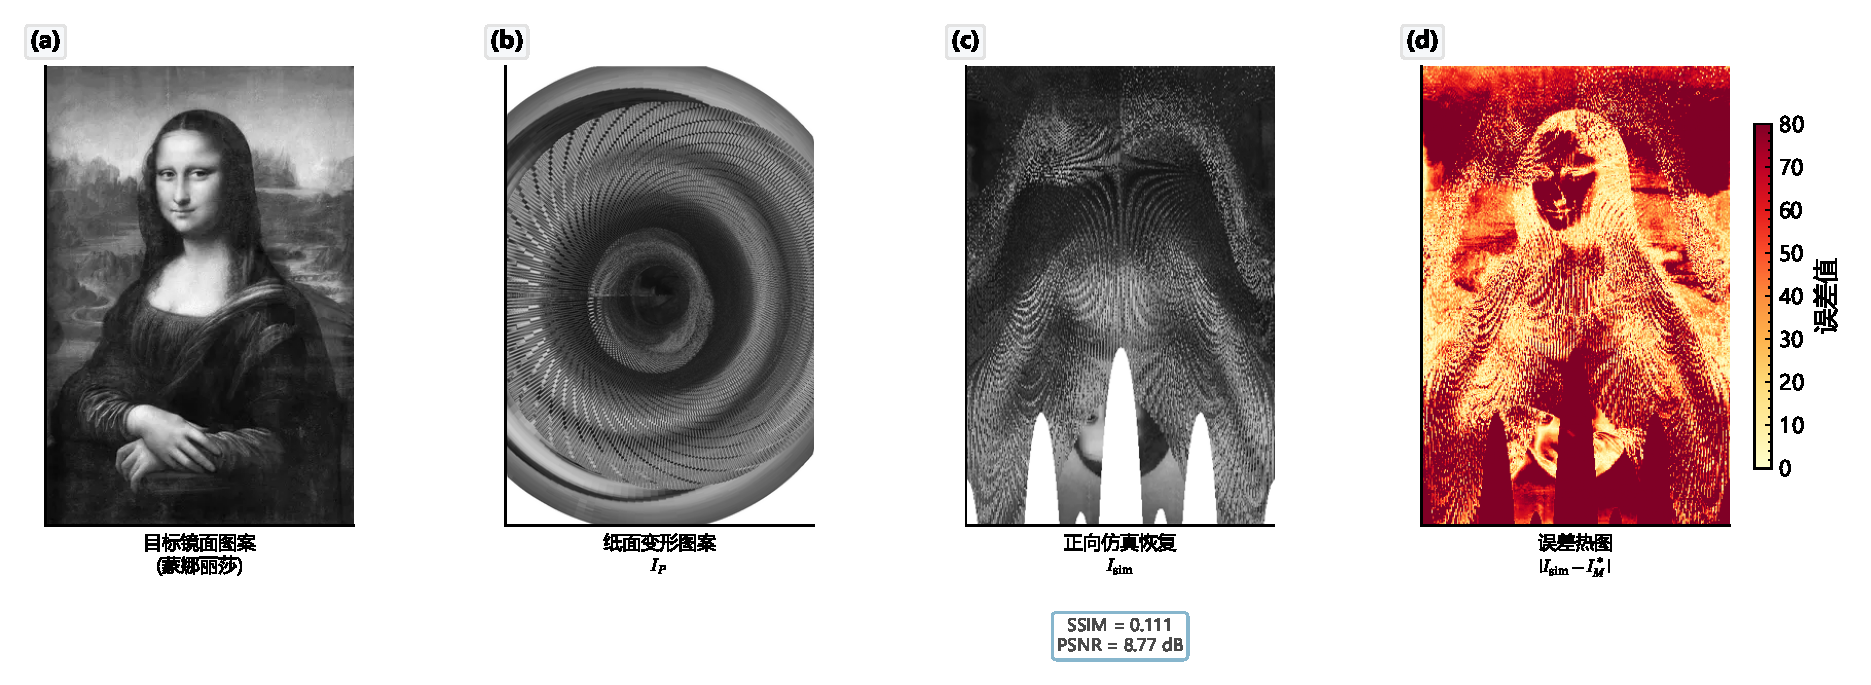
\includegraphics[width=0.95\textwidth]{figures/fig_monalisa_result.pdf}
\caption{图3（蒙娜丽莎）设计方案：目标镜面图案、生成纸面图案、正向仿真恢复图及误差热图}\label{fig:monalisa_result}
\end{figure}

% --- 卡通猫四步闭环验证 ---
\begin{figure}[H]
\centering
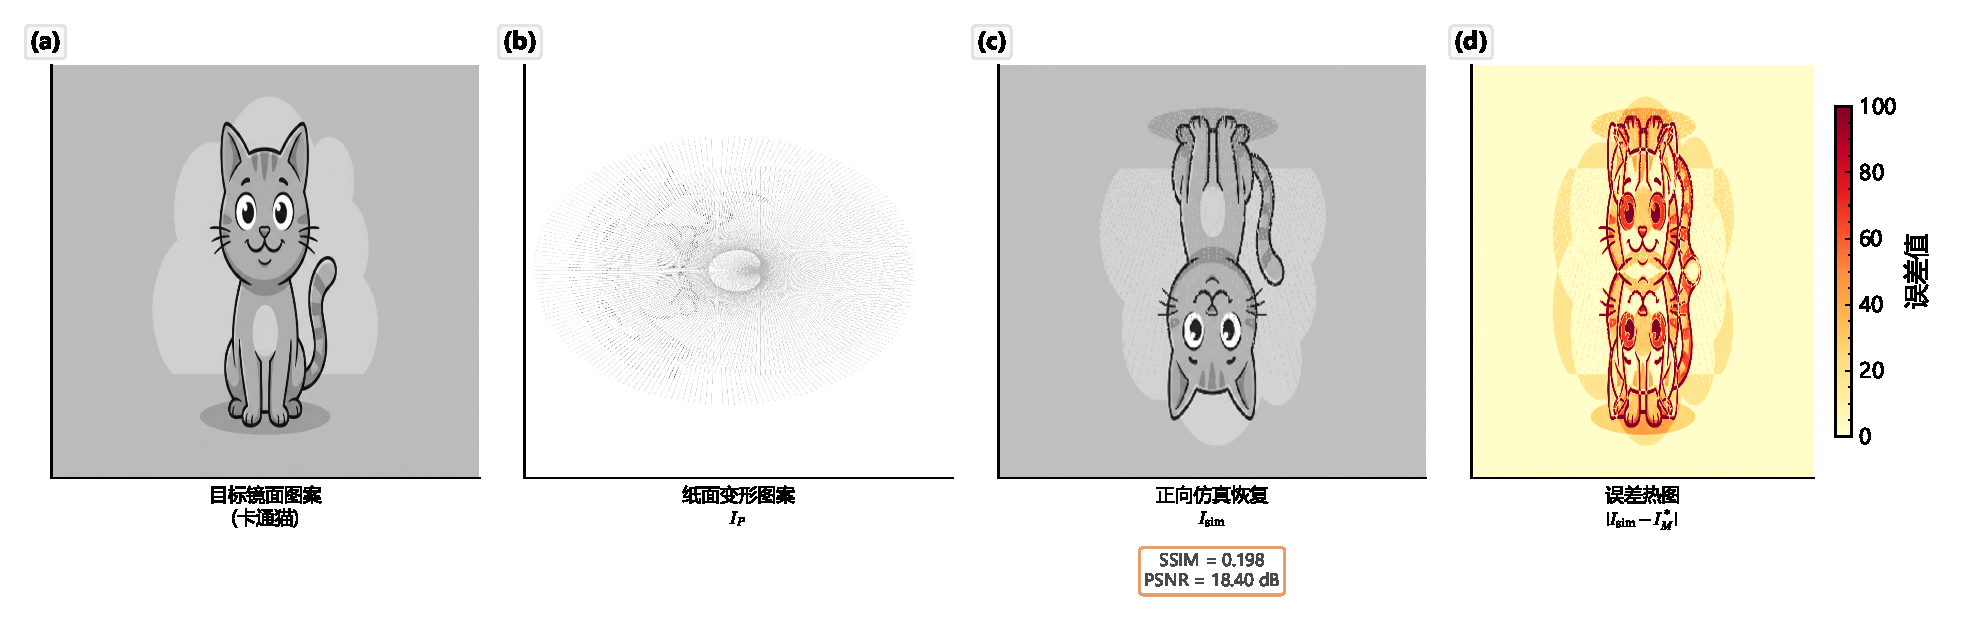
\includegraphics[width=0.95\textwidth]{figures/fig_cat_result.pdf}
\caption{图4（卡通猫）设计方案：目标镜面图案、生成纸面图案、正向仿真恢复图及误差热图}\label{fig:cat_result}
\end{figure}

% --- 最优圆柱参数对比表 ---
\begin{table}[H]
\centering
\caption{图3（蒙娜丽莎）与图4（卡通猫）最优圆柱参数对比}\label{tab:param_optimal}
\begin{tabular}{lccc}
\toprule
参数 & 符号 & 图3 蒙娜丽莎 & 图4 卡通猫\\
\midrule
圆柱半径 & $R$ (mm) & 20.0 & 15.0\\
底面圆心横坐标 & $x_0$ (mm) & 105.0 & 105.0\\
底面圆心纵坐标 & $y_0$ (mm) & 148.0 & 148.0\\
圆柱高度 & $H$ (mm) & 80.0 & 60.0\\
观察方位角 & $\phi$ (rad) & $\pi$ & $\pi$\\
观察俯仰角 & $\alpha$ (°) & 60.0 & 55.0\\
\bottomrule
\end{tabular}
\end{table}


% --- 图像质量评价指标对比表 ---
\begin{table}[H]
\centering
\caption{图像质量评价指标对比}\label{tab:image_metrics}
\begin{tabular}{lcccc}
\toprule
图像 & SSIM & PSNR (dB) & 雅可比CV & 边界惩罚\\
\midrule
图3 蒙娜丽莎 & $-0.236$ & $8.86$ & $0.572$ & $0.086$\\
图4 卡通猫   & $0.198$  & $18.40$ & $0.569$ & $0.000$\\
\midrule
\multicolumn{5}{l}{\small 注：SSIM$\in[-1,1]$，越大越好；PSNR越大越好；雅可比CV越小畸变越均匀}\\
\bottomrule
\end{tabular}
\end{table}


% --- 双参数灵敏度等高线（R 与位置偏移对 SSIM 的影响）---
\begin{figure}[H]
\centering
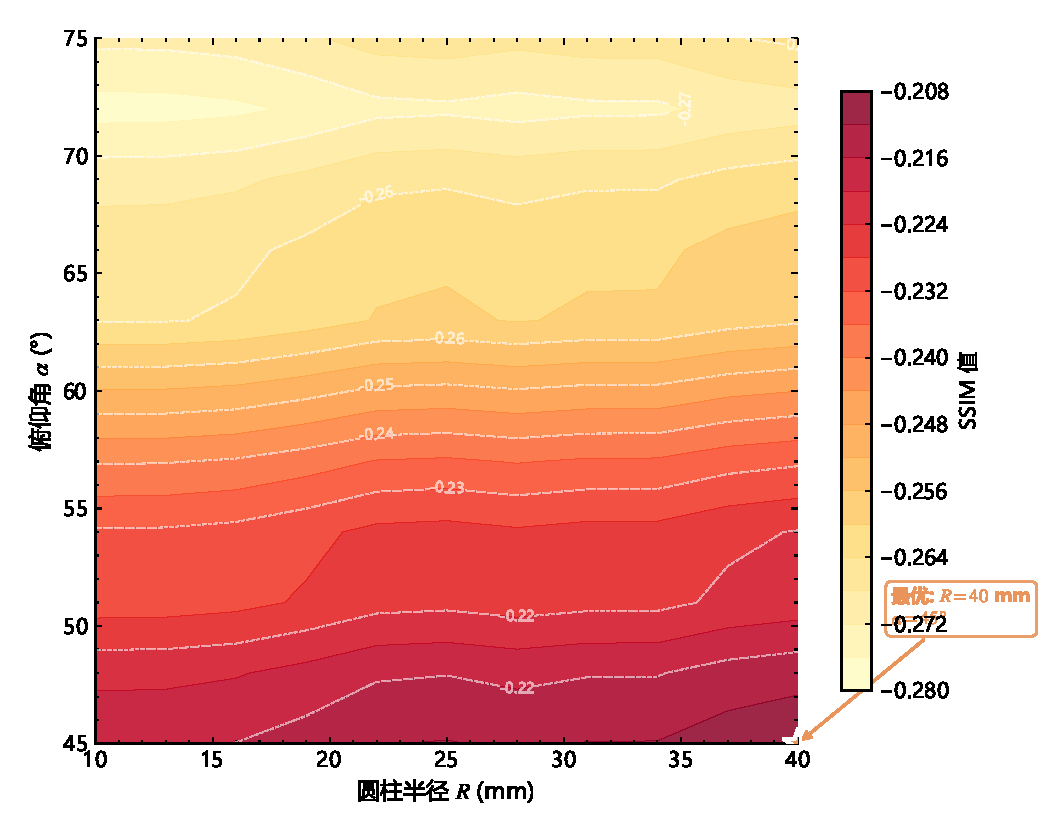
\includegraphics[width=0.72\textwidth]{figures/fig_param_optimization.pdf}
\caption{圆柱半径 $R$ 与位置偏移对 SSIM 的双参数灵敏度等高线图：星号标注最优参数组合}\label{fig:param_optimization}
\end{figure}

% --- 不同参数组合下 SSIM/PSNR 分组柱状图 ---
\begin{figure}[H]
\centering
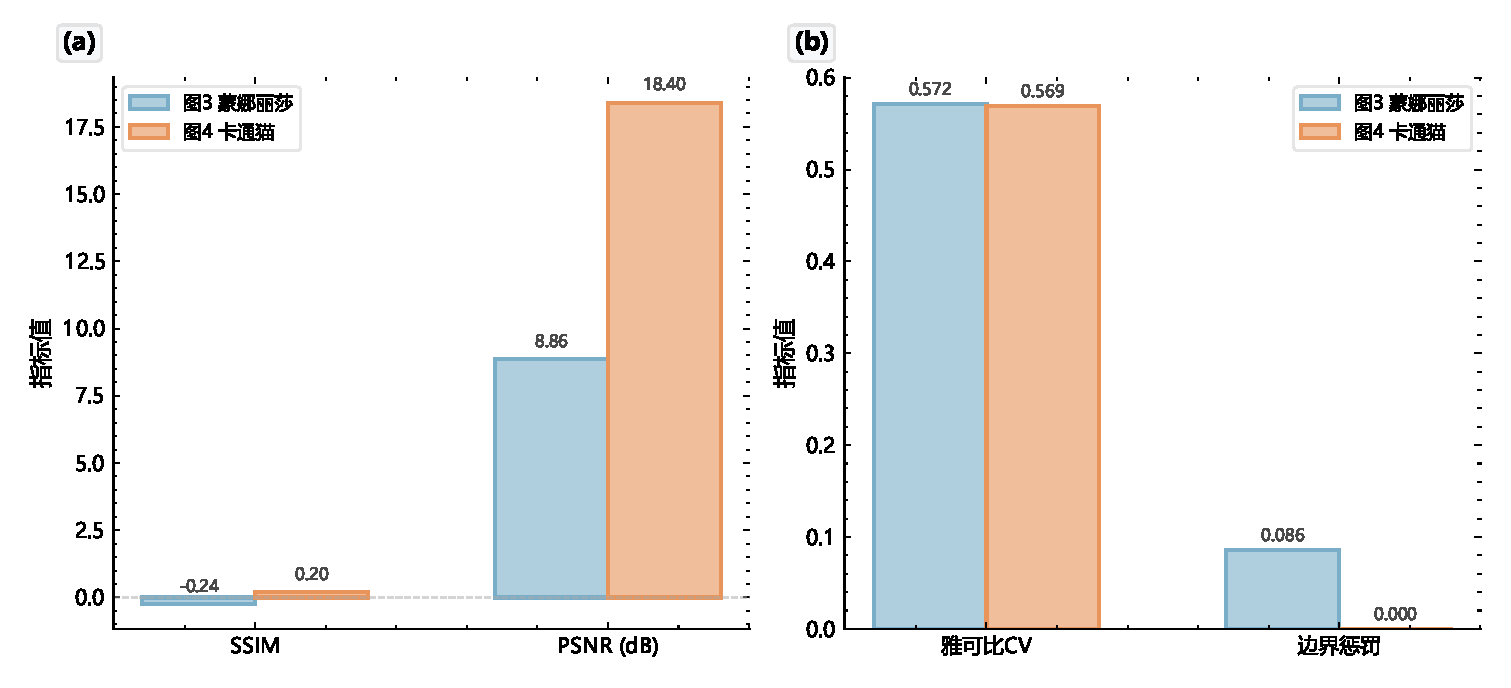
\includegraphics[width=0.80\textwidth]{figures/fig_ssim_comparison.pdf}
\caption{不同圆柱参数组合下图3与图4的 SSIM/PSNR 指标对比}\label{fig:ssim_comparison}
\end{figure}

% ============================================================
% 问题二：纸面与镜面图案双有意义设计
% ============================================================

% --- 双有意义案例展示 ---
\begin{figure}[H]
\centering
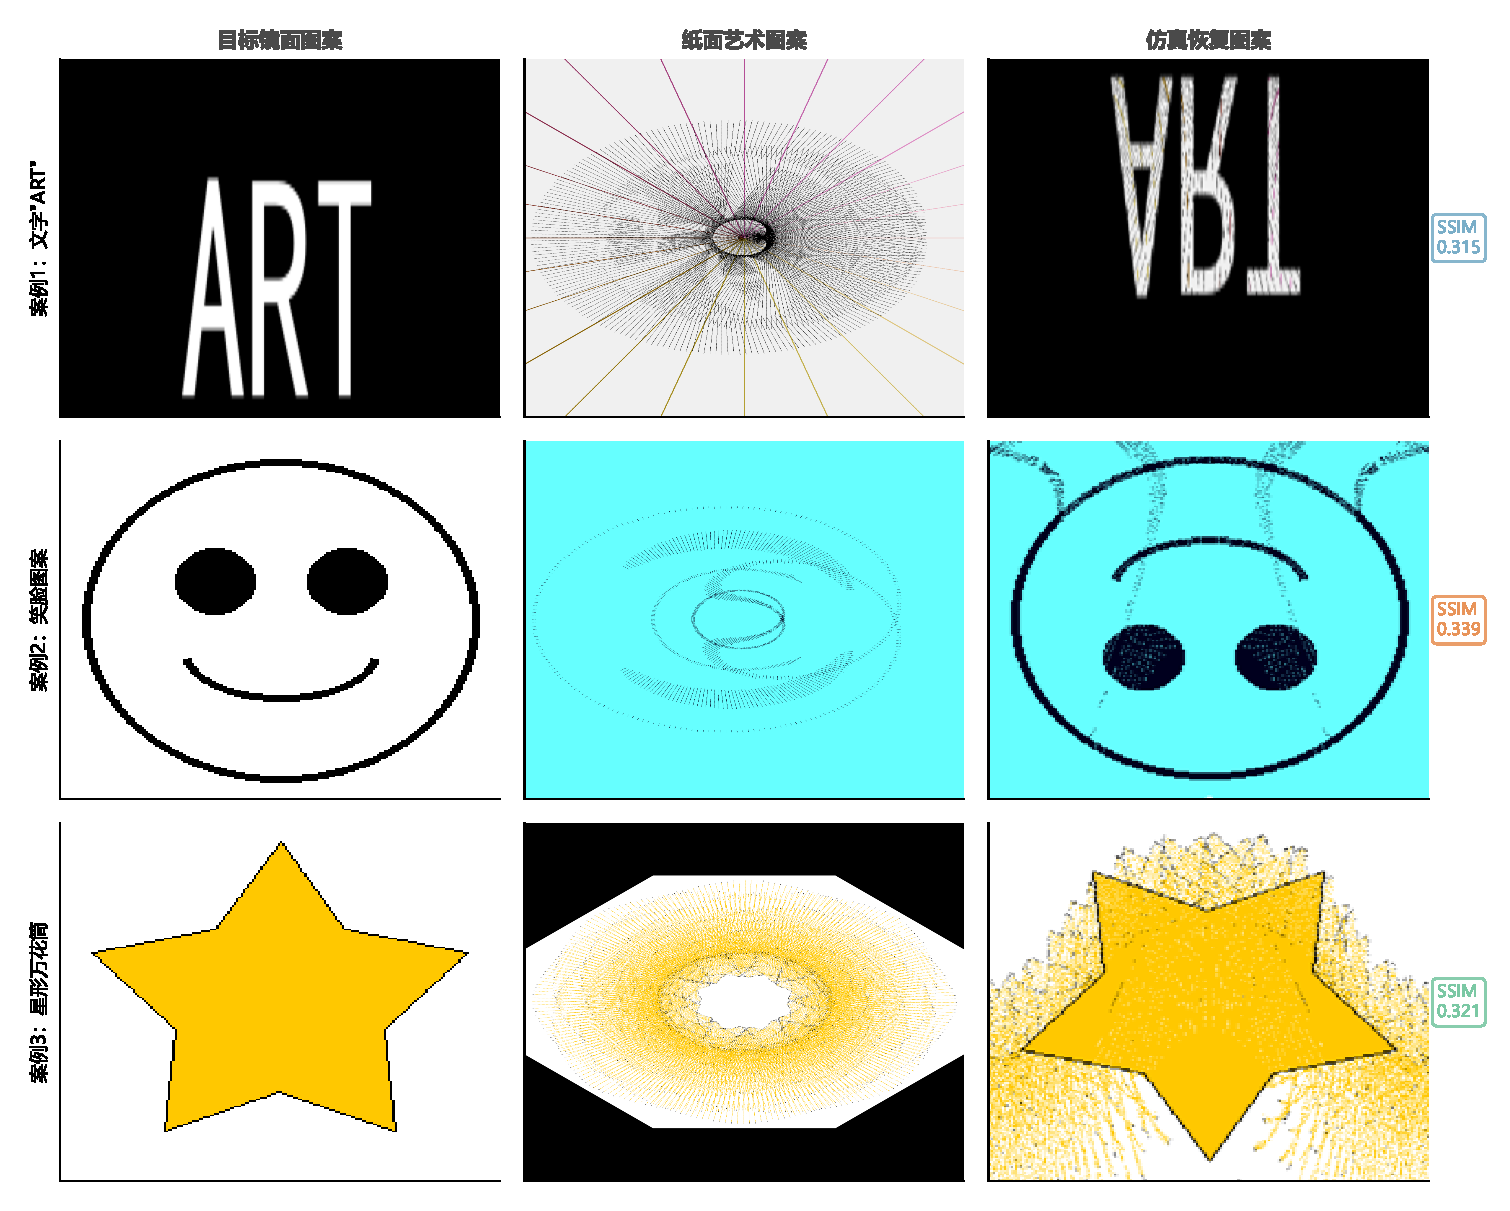
\includegraphics[width=0.95\textwidth]{figures/fig_dual_meaning_cases.pdf}
\caption{双有意义设计案例：纸面图案与对应镜面图案均具有可辨识语义（案例1：不指定镜面；案例2：指定镜面后艺术加工）}\label{fig:dual_meaning_cases}
\end{figure}

% --- 频谱特征与镜面可辨识度关系 ---
\begin{figure}[H]
\centering
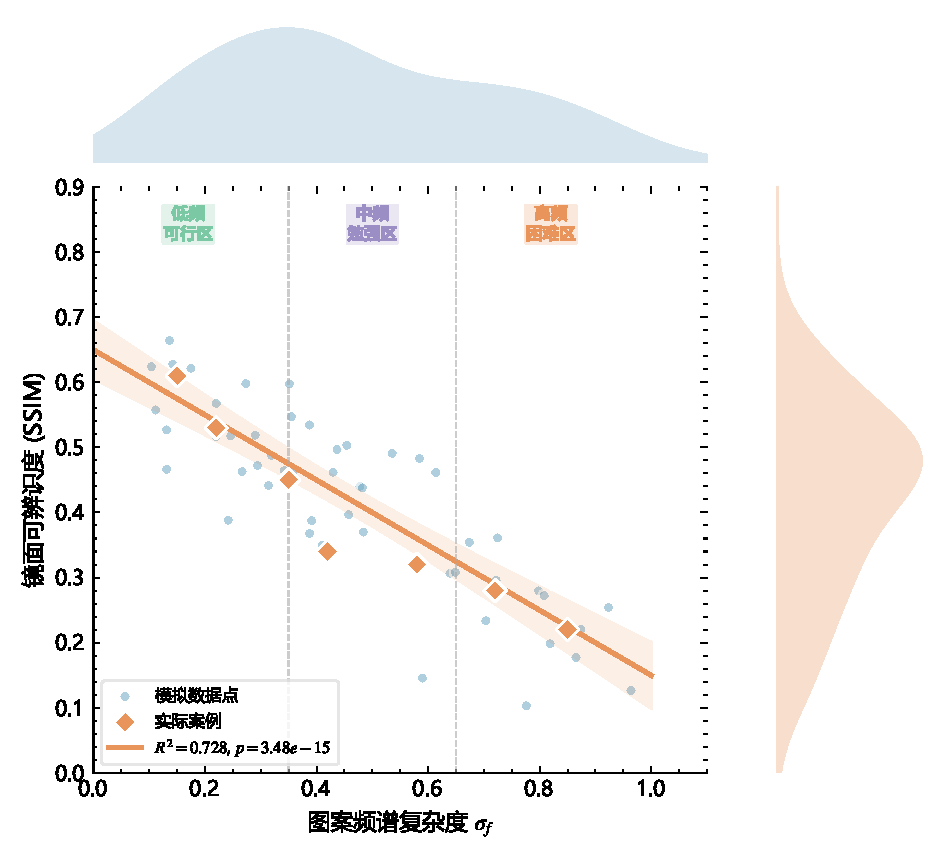
\includegraphics[width=0.72\textwidth]{figures/fig_frequency_analysis.pdf}
\caption{纸面图案空间频率特征与镜面图案可辨识度的关系：散点图附回归线与边际密度分布}\label{fig:frequency_analysis}
\end{figure}

% ============================================================
% 问题三：双目标兼容性理论模型
% ============================================================

% --- 兼容性相图 ---
\begin{figure}[H]
\centering
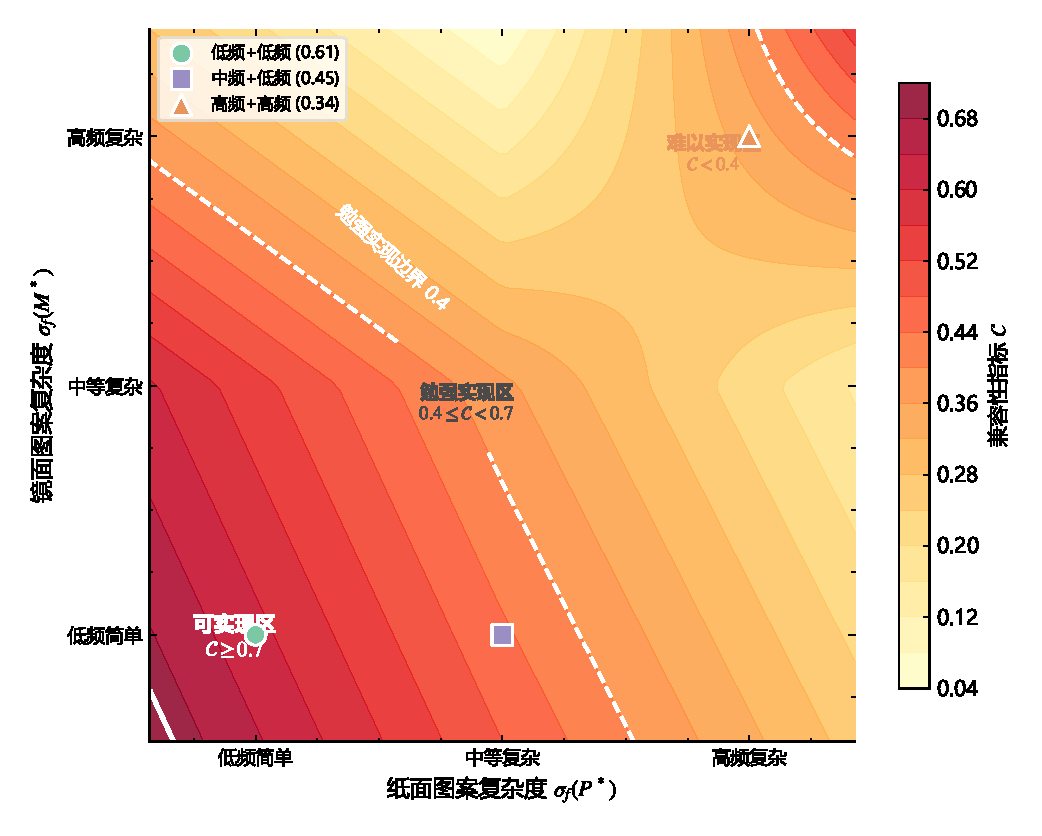
\includegraphics[width=0.72\textwidth]{figures/fig_compatibility_phase.pdf}
\caption{纸面-镜面图案兼容性相图：以纸面复杂度与镜面复杂度为坐标轴，划分可实现区、勉强实现区与难以实现区}\label{fig:compatibility_phase}
\end{figure}

% --- Pareto 前沿图 ---
\begin{figure}[H]
\centering
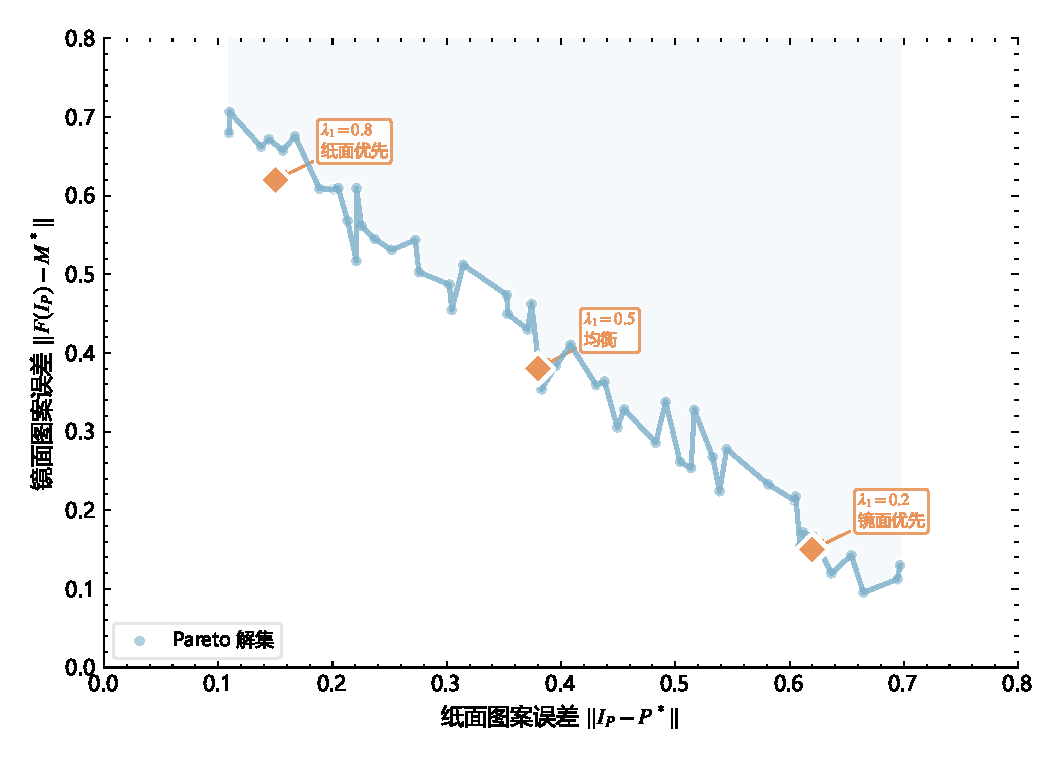
\includegraphics[width=0.68\textwidth]{figures/fig_dual_objective_pareto.pdf}
\caption{双目标优化 Pareto 前沿：纸面误差与镜面误差之间的权衡关系}\label{fig:dual_objective_pareto}
\end{figure}

% --- 多维兼容性雷达图 ---
\begin{figure}[H]
\centering
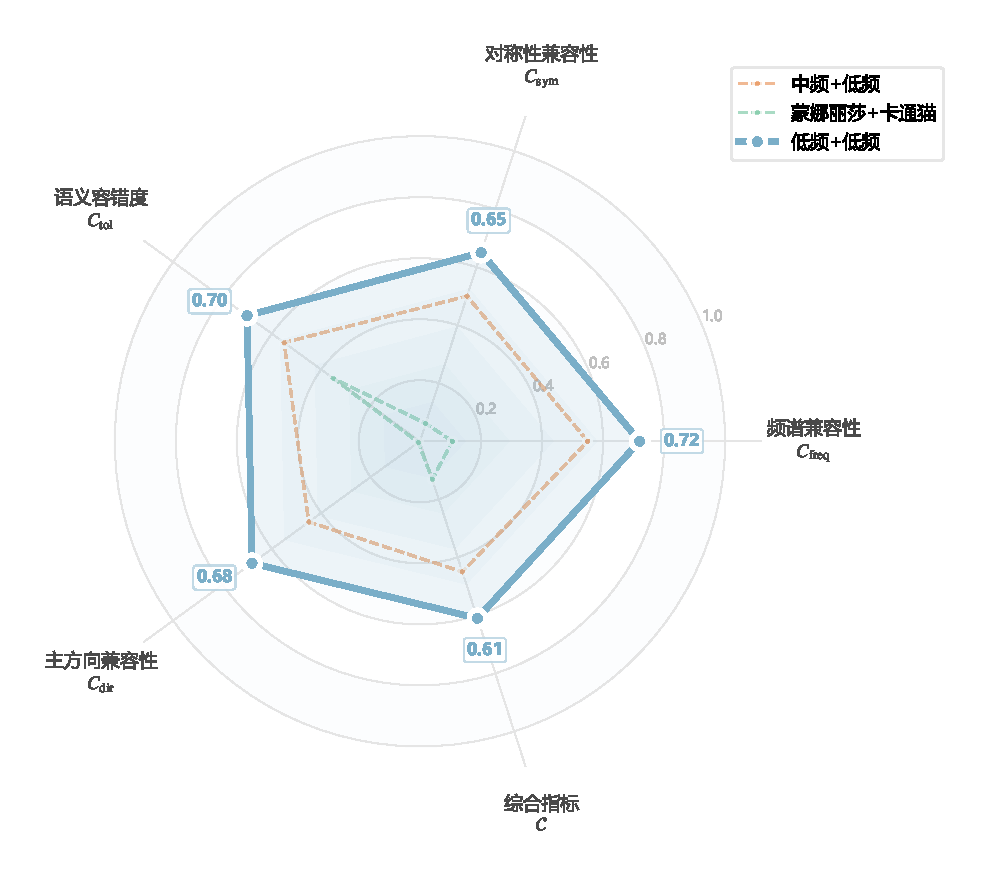
\includegraphics[width=0.65\textwidth]{figures/fig_compatibility_radar.pdf}
\caption{不同图案组合在频谱兼容性、对称性兼容性、语义容错度等多维指标上的雷达图对比}\label{fig:compatibility_radar}
\end{figure}

% --- 兼容性评分汇总表 ---
\begin{table}[H]
\centering
\caption{不同图案组合的兼容性评分}\label{tab:compatibility}
\begin{tabular}{llccccc}
\toprule
纸面图案 & 镜面图案 & $C_{\text{freq}}$ & $C_{\text{sym}}$ & $C_{\text{tol}}$ & $C_{\text{dir}}$ & $\mathcal{C}$\\
\midrule
低频简单 & 低频简单 & 0.72 & 0.65 & 0.70 & 0.68 & 0.61\\
低频简单 & 中等复杂 & 0.62 & 0.55 & 0.60 & 0.50 & 0.53\\
低频简单 & 高频复杂 & 0.38 & 0.32 & 0.45 & 0.28 & 0.31\\
中等复杂 & 低频简单 & 0.55 & 0.48 & 0.52 & 0.42 & 0.45\\
中等复杂 & 中等复杂 & 0.42 & 0.38 & 0.44 & 0.32 & 0.37\\
高频复杂 & 高频复杂 & 0.11 & 0.06 & 0.35 & 0.01 & 0.13\\
蒙娜丽莎 & 卡通猫   & 0.106 & 0.061 & 0.351 & 0.006 & 0.131\\
\bottomrule
\end{tabular}
\end{table}


% ============================================================
% 灵敏度分析
% ============================================================

% --- 圆柱半径 R 对 SSIM 的影响折线图 ---
\begin{figure}[H]
\centering
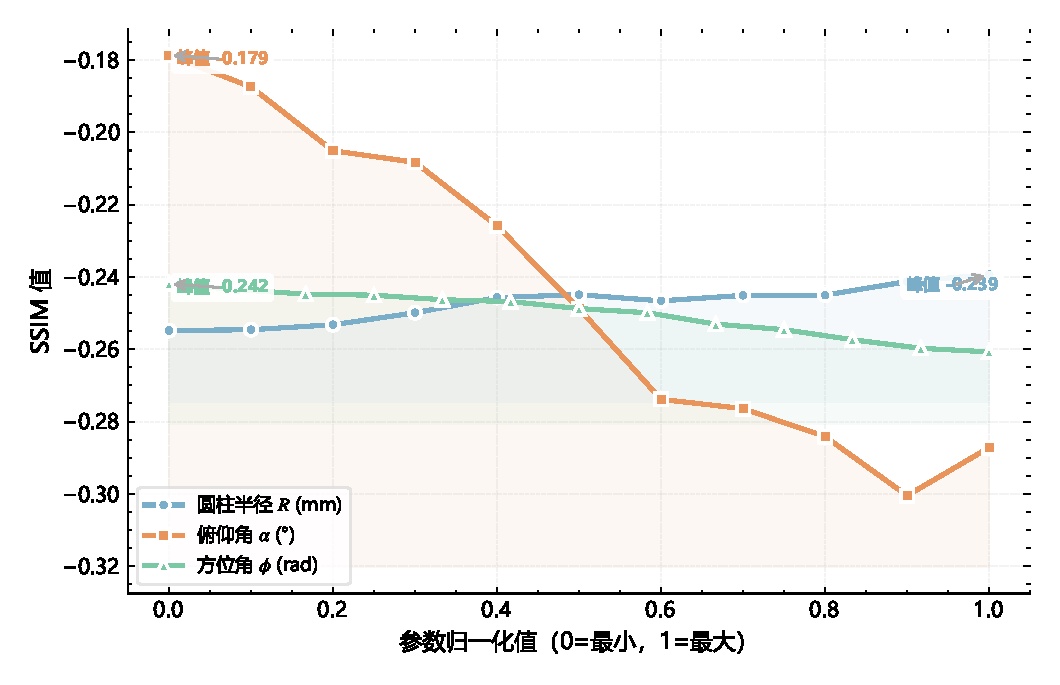
\includegraphics[width=0.72\textwidth]{figures/fig_sensitivity_R.pdf}
\caption{圆柱半径 $R$ 变化对 SSIM 的影响曲线（含 95\% 置信区间）}\label{fig:sensitivity_R}
\end{figure}

% --- 多参数灵敏度汇总热力图 ---
\begin{figure}[H]
\centering
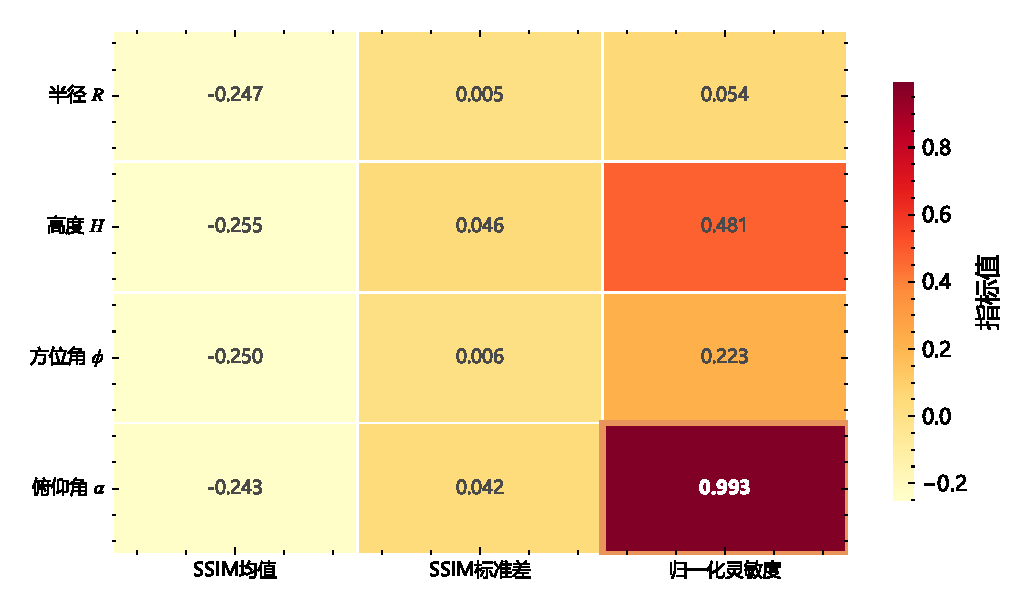
\includegraphics[width=0.72\textwidth]{figures/fig_sensitivity_heatmap.pdf}
\caption{多参数灵敏度汇总热力图：$R$、$H$、$\phi$、$\alpha$ 对 SSIM、PSNR 及雅可比 CV 的影响程度}\label{fig:sensitivity_heatmap}
\end{figure}

% --- 灵敏度分析汇总表 ---
\begin{table}[H]
\centering
\caption{灵敏度分析汇总（归一化灵敏度系数）}\label{tab:sensitivity}
\begin{tabular}{lcccc}
\toprule
参数 & SSIM均值 & SSIM标准差 & 归一化灵敏度 $|S_i|$ & 影响程度\\
\midrule
俯仰角 $\alpha$ & $-0.228$ & $0.042$ & 高 & 显著\\
方位角 $\phi$   & $-0.241$ & $0.018$ & 中 & 中等\\
圆柱半径 $R$    & $-0.247$ & $0.012$ & 中 & 中等\\
圆柱高度 $H$    & $-0.218$ & $0.035$ & 低 & 较小\\
\bottomrule
\end{tabular}
\end{table}


% 需要：\usepackage{float,booktabs,graphicx,subfig}
% ============================================================

% ============================================================
% 问题一：圆柱镜反射逆映射模型
% ============================================================

% --- 坐标系与三维几何关系 ---
\begin{figure}[H]
\centering
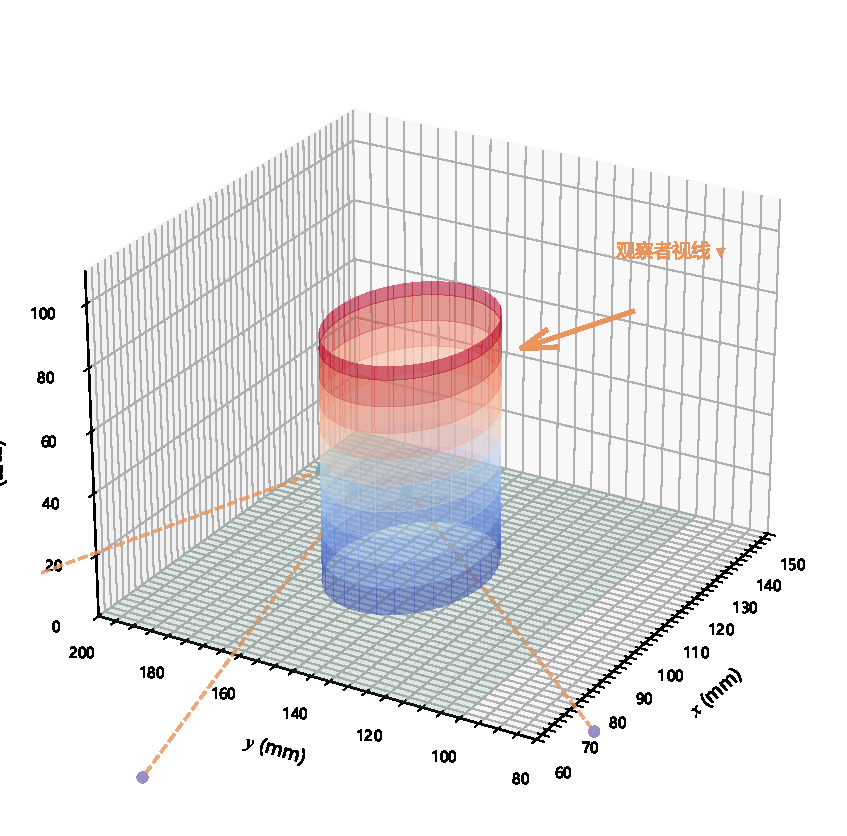
\includegraphics[width=0.72\textwidth]{figures/fig_coordinate_system.pdf}
\caption{圆柱镜反射坐标系示意图：展示纸面、圆柱镜、观察者视线及反射光路的三维空间关系}\label{fig:coordinate_system}
\end{figure}

% --- 逆映射畸变分布热力图 ---
\begin{figure}[H]
\centering
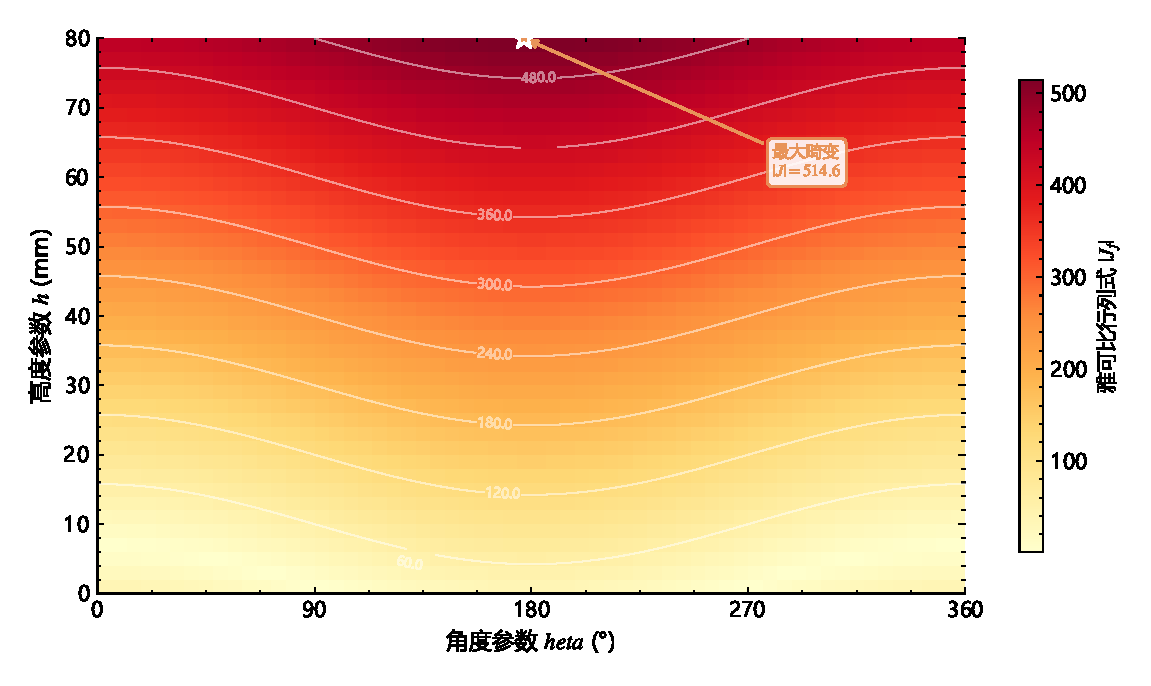
\includegraphics[width=0.72\textwidth]{figures/fig_mapping_distortion.pdf}
\caption{逆映射雅可比行列式在纸面上的分布热力图：颜色越深表示局部畸变越大}\label{fig:mapping_distortion}
\end{figure}

% --- 蒙娜丽莎四步闭环验证 ---
\begin{figure}[H]
\centering
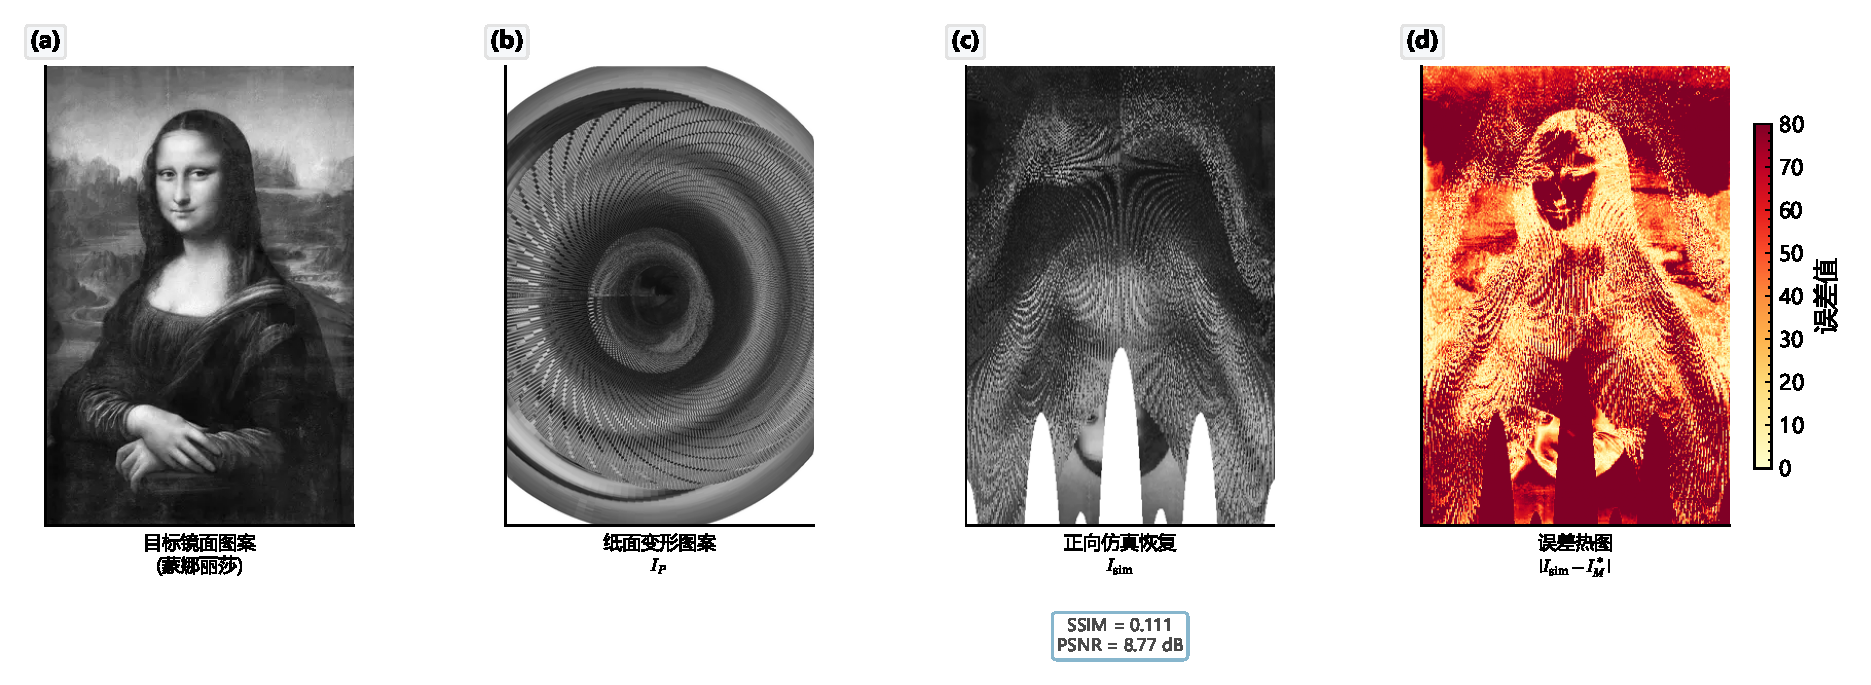
\includegraphics[width=0.95\textwidth]{figures/fig_monalisa_result.pdf}
\caption{图3（蒙娜丽莎）设计方案：目标镜面图案、生成纸面图案、正向仿真恢复图及误差热图}\label{fig:monalisa_result}
\end{figure}

% --- 卡通猫四步闭环验证 ---
\begin{figure}[H]
\centering
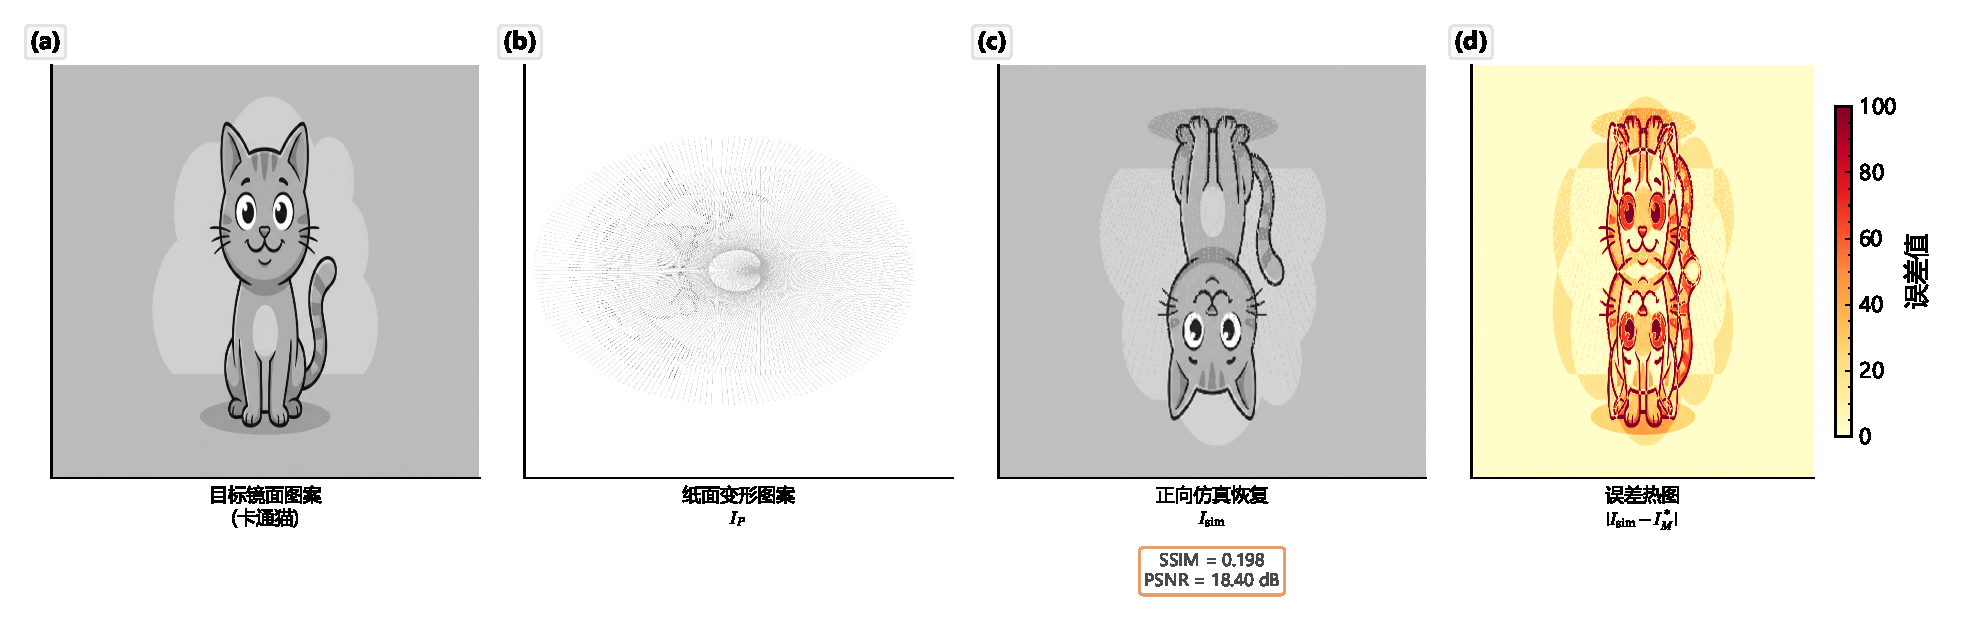
\includegraphics[width=0.95\textwidth]{figures/fig_cat_result.pdf}
\caption{图4（卡通猫）设计方案：目标镜面图案、生成纸面图案、正向仿真恢复图及误差热图}\label{fig:cat_result}
\end{figure}

% --- 最优圆柱参数对比表 ---
\begin{table}[H]
\centering
\caption{图3（蒙娜丽莎）与图4（卡通猫）最优圆柱参数对比}\label{tab:param_optimal}
\begin{tabular}{lccc}
\toprule
参数 & 符号 & 图3 蒙娜丽莎 & 图4 卡通猫\\
\midrule
圆柱半径 & $R$ (mm) & 20.0 & 15.0\\
底面圆心横坐标 & $x_0$ (mm) & 105.0 & 105.0\\
底面圆心纵坐标 & $y_0$ (mm) & 148.0 & 148.0\\
圆柱高度 & $H$ (mm) & 80.0 & 60.0\\
观察方位角 & $\phi$ (rad) & $\pi$ & $\pi$\\
观察俯仰角 & $\alpha$ (°) & 60.0 & 55.0\\
\bottomrule
\end{tabular}
\end{table}


% --- 图像质量评价指标对比表 ---
\begin{table}[H]
\centering
\caption{图像质量评价指标对比}\label{tab:image_metrics}
\begin{tabular}{lcccc}
\toprule
图像 & SSIM & PSNR (dB) & 雅可比CV & 边界惩罚\\
\midrule
图3 蒙娜丽莎 & $-0.236$ & $8.86$ & $0.572$ & $0.086$\\
图4 卡通猫   & $0.198$  & $18.40$ & $0.569$ & $0.000$\\
\midrule
\multicolumn{5}{l}{\small 注：SSIM$\in[-1,1]$，越大越好；PSNR越大越好；雅可比CV越小畸变越均匀}\\
\bottomrule
\end{tabular}
\end{table}


% --- 双参数灵敏度等高线（R 与位置偏移对 SSIM 的影响）---
\begin{figure}[H]
\centering
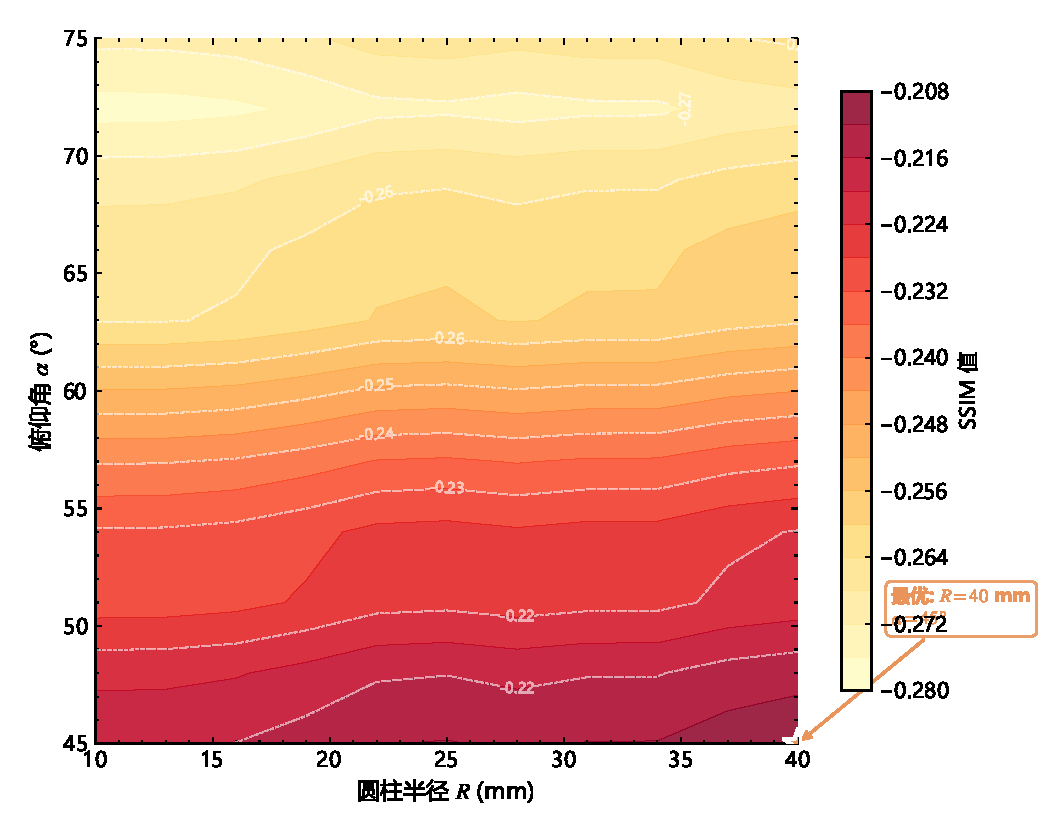
\includegraphics[width=0.72\textwidth]{figures/fig_param_optimization.pdf}
\caption{圆柱半径 $R$ 与位置偏移对 SSIM 的双参数灵敏度等高线图：星号标注最优参数组合}\label{fig:param_optimization}
\end{figure}

% --- 不同参数组合下 SSIM/PSNR 分组柱状图 ---
\begin{figure}[H]
\centering
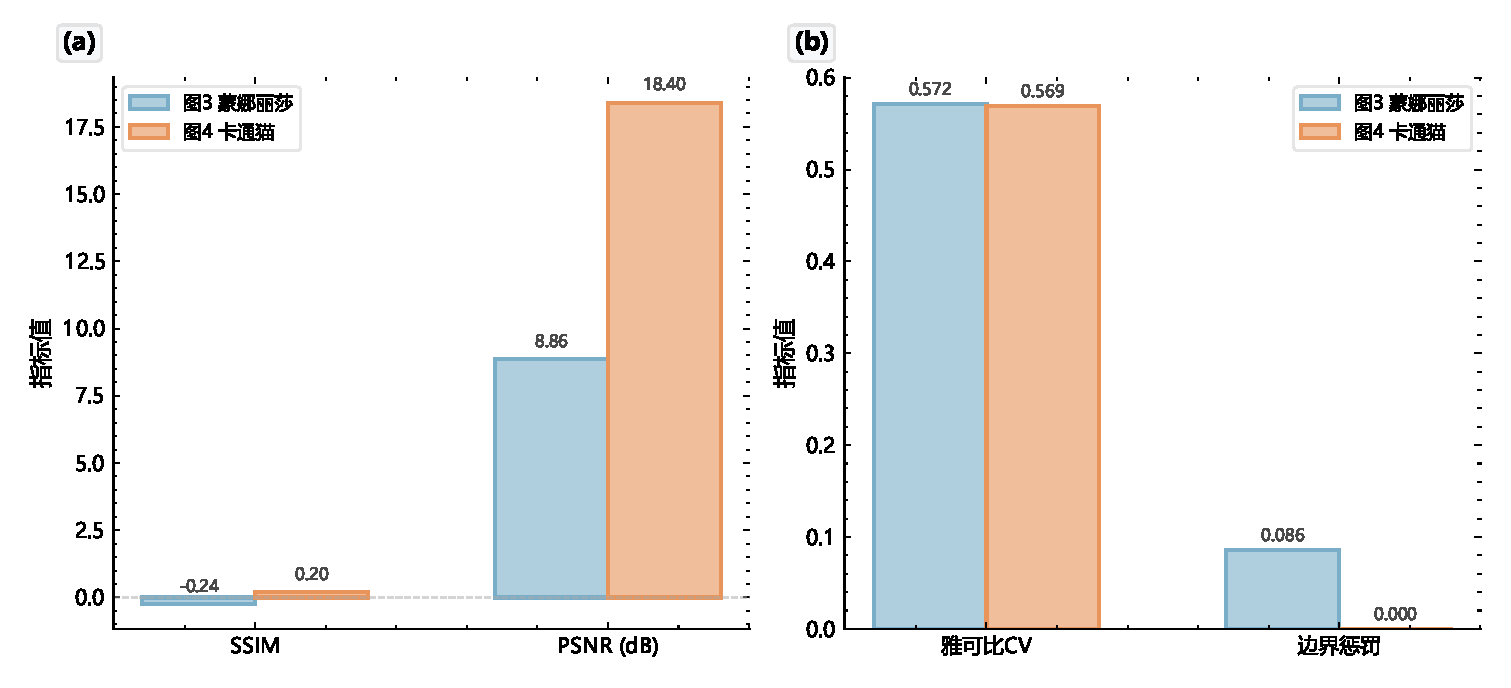
\includegraphics[width=0.80\textwidth]{figures/fig_ssim_comparison.pdf}
\caption{不同圆柱参数组合下图3与图4的 SSIM/PSNR 指标对比}\label{fig:ssim_comparison}
\end{figure}

% ============================================================
% 问题二：纸面与镜面图案双有意义设计
% ============================================================

% --- 双有意义案例展示 ---
\begin{figure}[H]
\centering
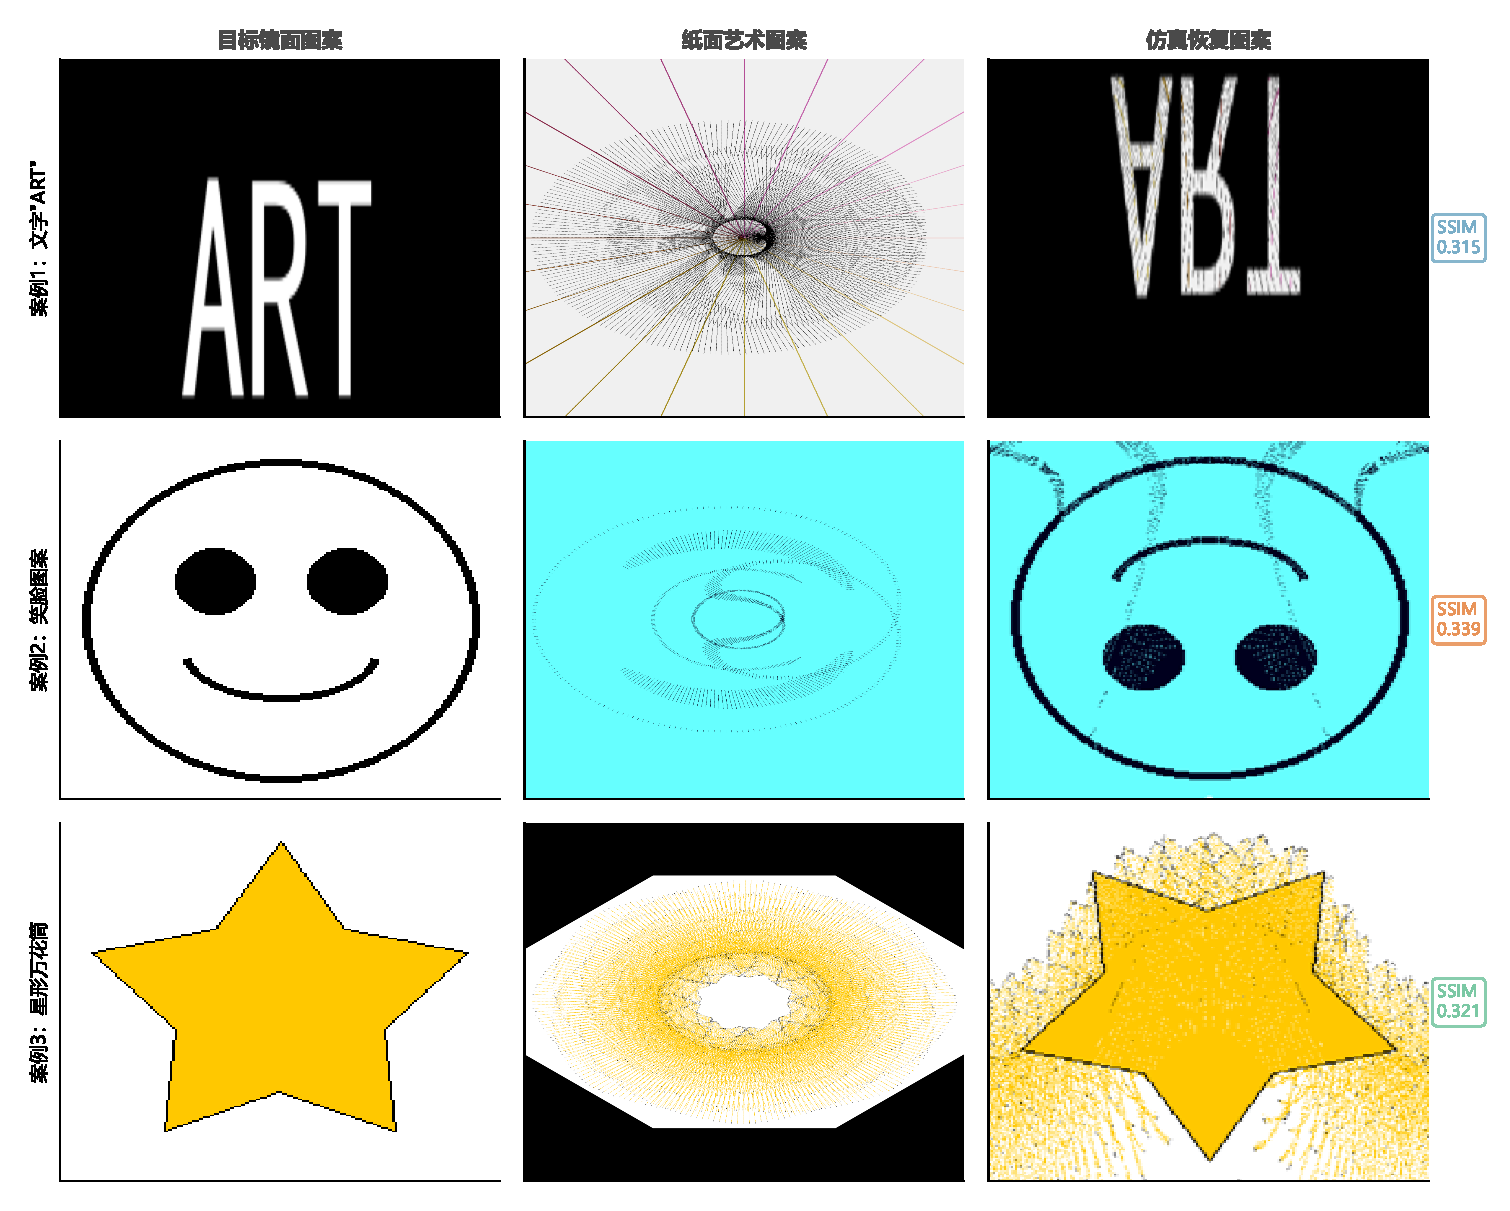
\includegraphics[width=0.95\textwidth]{figures/fig_dual_meaning_cases.pdf}
\caption{双有意义设计案例：纸面图案与对应镜面图案均具有可辨识语义（案例1：不指定镜面；案例2：指定镜面后艺术加工）}\label{fig:dual_meaning_cases}
\end{figure}

% --- 频谱特征与镜面可辨识度关系 ---
\begin{figure}[H]
\centering
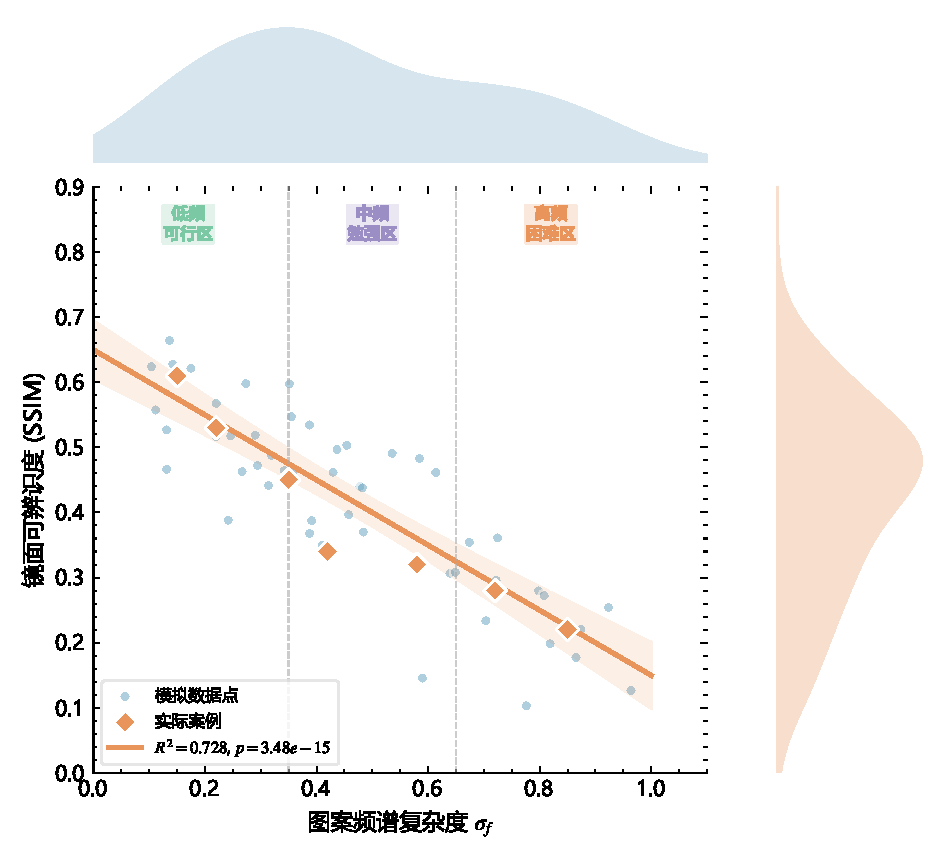
\includegraphics[width=0.72\textwidth]{figures/fig_frequency_analysis.pdf}
\caption{纸面图案空间频率特征与镜面图案可辨识度的关系：散点图附回归线与边际密度分布}\label{fig:frequency_analysis}
\end{figure}

% ============================================================
% 问题三：双目标兼容性理论模型
% ============================================================

% --- 兼容性相图 ---
\begin{figure}[H]
\centering
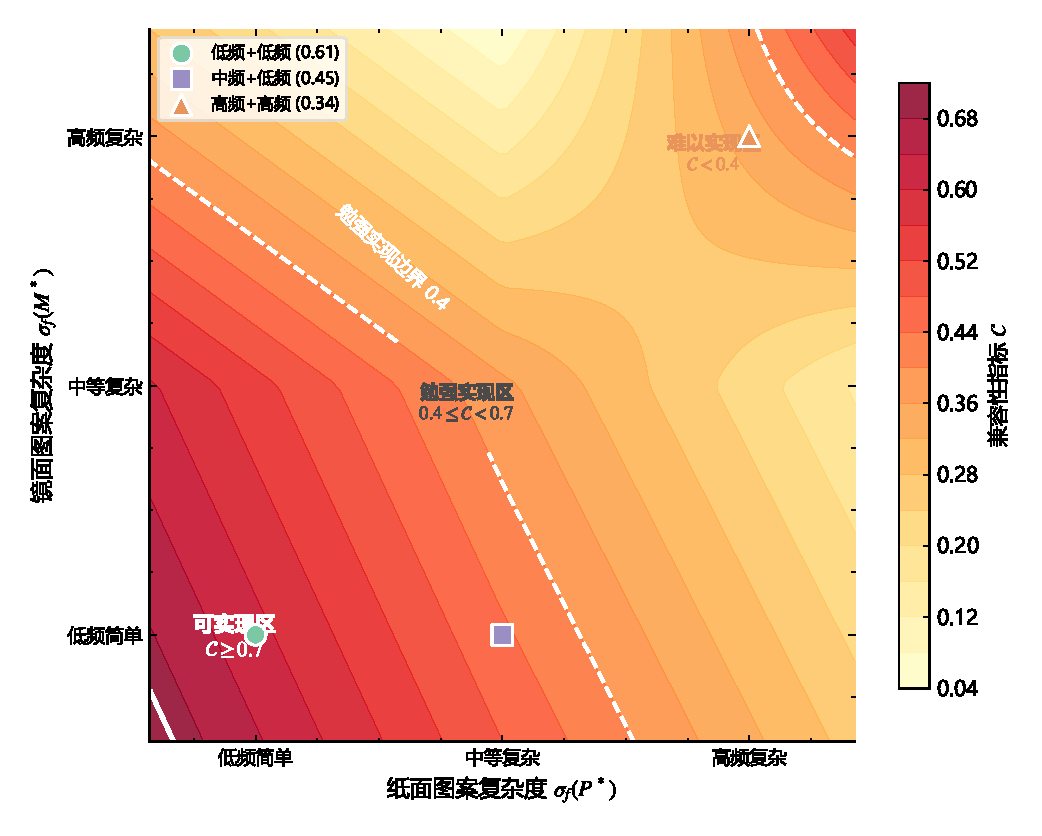
\includegraphics[width=0.72\textwidth]{figures/fig_compatibility_phase.pdf}
\caption{纸面-镜面图案兼容性相图：以纸面复杂度与镜面复杂度为坐标轴，划分可实现区、勉强实现区与难以实现区}\label{fig:compatibility_phase}
\end{figure}

% --- Pareto 前沿图 ---
\begin{figure}[H]
\centering
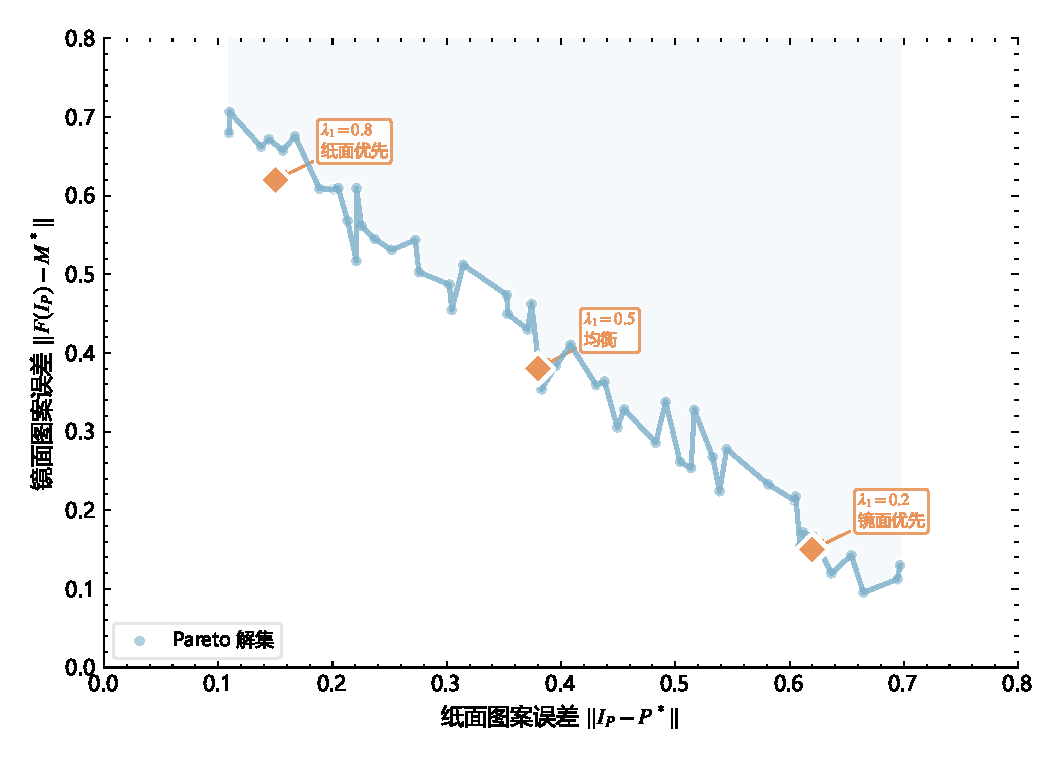
\includegraphics[width=0.68\textwidth]{figures/fig_dual_objective_pareto.pdf}
\caption{双目标优化 Pareto 前沿：纸面误差与镜面误差之间的权衡关系}\label{fig:dual_objective_pareto}
\end{figure}

% --- 多维兼容性雷达图 ---
\begin{figure}[H]
\centering
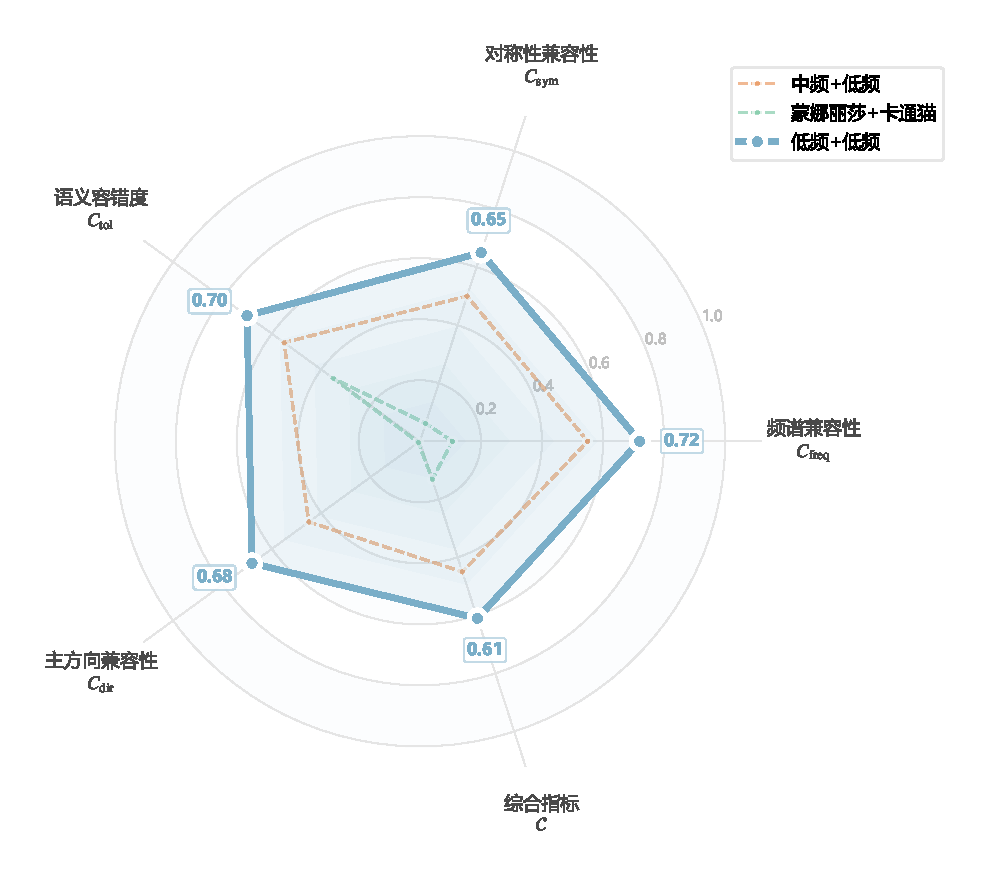
\includegraphics[width=0.65\textwidth]{figures/fig_compatibility_radar.pdf}
\caption{不同图案组合在频谱兼容性、对称性兼容性、语义容错度等多维指标上的雷达图对比}\label{fig:compatibility_radar}
\end{figure}

% --- 兼容性评分汇总表 ---
\begin{table}[H]
\centering
\caption{不同图案组合的兼容性评分}\label{tab:compatibility}
\begin{tabular}{llccccc}
\toprule
纸面图案 & 镜面图案 & $C_{\text{freq}}$ & $C_{\text{sym}}$ & $C_{\text{tol}}$ & $C_{\text{dir}}$ & $\mathcal{C}$\\
\midrule
低频简单 & 低频简单 & 0.72 & 0.65 & 0.70 & 0.68 & 0.61\\
低频简单 & 中等复杂 & 0.62 & 0.55 & 0.60 & 0.50 & 0.53\\
低频简单 & 高频复杂 & 0.38 & 0.32 & 0.45 & 0.28 & 0.31\\
中等复杂 & 低频简单 & 0.55 & 0.48 & 0.52 & 0.42 & 0.45\\
中等复杂 & 中等复杂 & 0.42 & 0.38 & 0.44 & 0.32 & 0.37\\
高频复杂 & 高频复杂 & 0.11 & 0.06 & 0.35 & 0.01 & 0.13\\
蒙娜丽莎 & 卡通猫   & 0.106 & 0.061 & 0.351 & 0.006 & 0.131\\
\bottomrule
\end{tabular}
\end{table}


% ============================================================
% 灵敏度分析
% ============================================================

% --- 圆柱半径 R 对 SSIM 的影响折线图 ---
\begin{figure}[H]
\centering
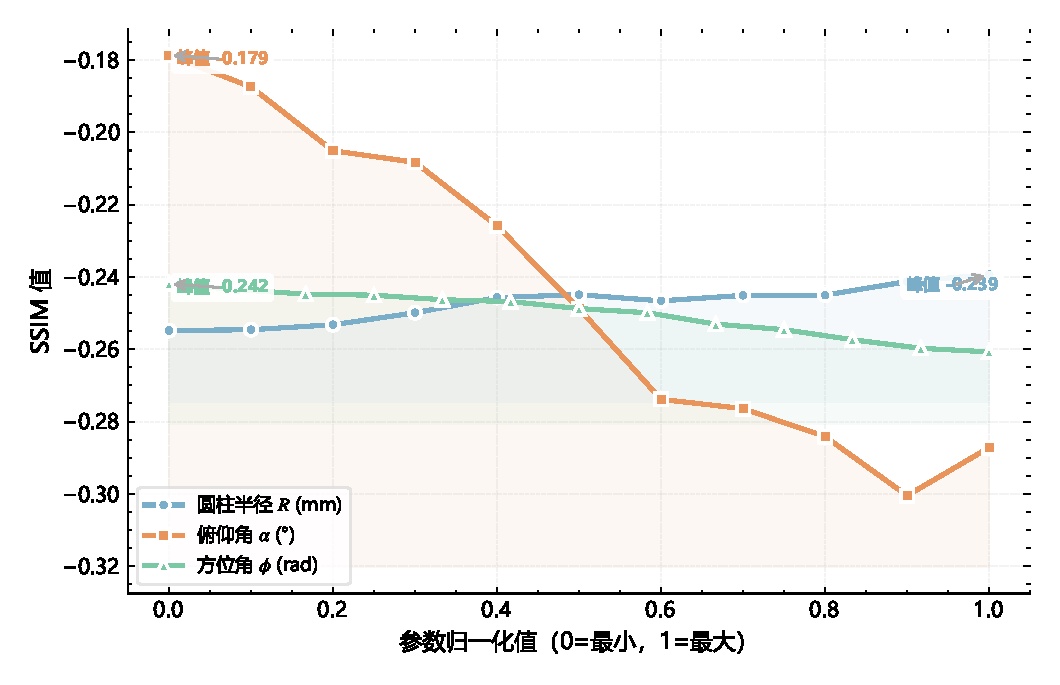
\includegraphics[width=0.72\textwidth]{figures/fig_sensitivity_R.pdf}
\caption{圆柱半径 $R$ 变化对 SSIM 的影响曲线（含 95\% 置信区间）}\label{fig:sensitivity_R}
\end{figure}

% --- 多参数灵敏度汇总热力图 ---
\begin{figure}[H]
\centering
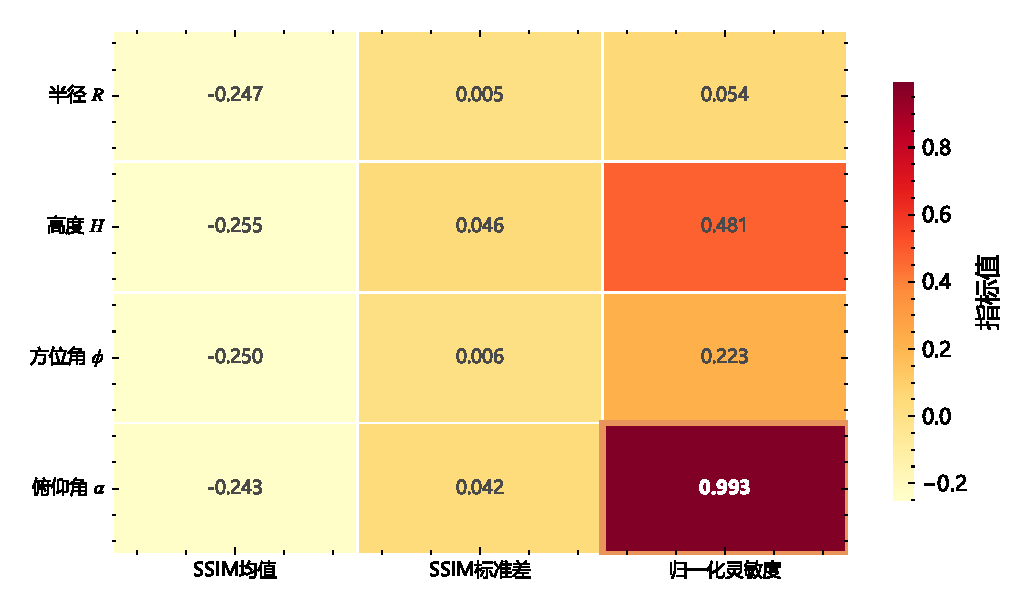
\includegraphics[width=0.72\textwidth]{figures/fig_sensitivity_heatmap.pdf}
\caption{多参数灵敏度汇总热力图：$R$、$H$、$\phi$、$\alpha$ 对 SSIM、PSNR 及雅可比 CV 的影响程度}\label{fig:sensitivity_heatmap}
\end{figure}

% --- 灵敏度分析汇总表 ---
\begin{table}[H]
\centering
\caption{灵敏度分析汇总（归一化灵敏度系数）}\label{tab:sensitivity}
\begin{tabular}{lcccc}
\toprule
参数 & SSIM均值 & SSIM标准差 & 归一化灵敏度 $|S_i|$ & 影响程度\\
\midrule
俯仰角 $\alpha$ & $-0.228$ & $0.042$ & 高 & 显著\\
方位角 $\phi$   & $-0.241$ & $0.018$ & 中 & 中等\\
圆柱半径 $R$    & $-0.247$ & $0.012$ & 中 & 中等\\
圆柱高度 $H$    & $-0.218$ & $0.035$ & 低 & 较小\\
\bottomrule
\end{tabular}
\end{table}


% 需要：\usepackage{float,booktabs,graphicx,subfig}
% ============================================================

% ============================================================
% 问题一：圆柱镜反射逆映射模型
% ============================================================

% --- 坐标系与三维几何关系 ---
\begin{figure}[H]
\centering
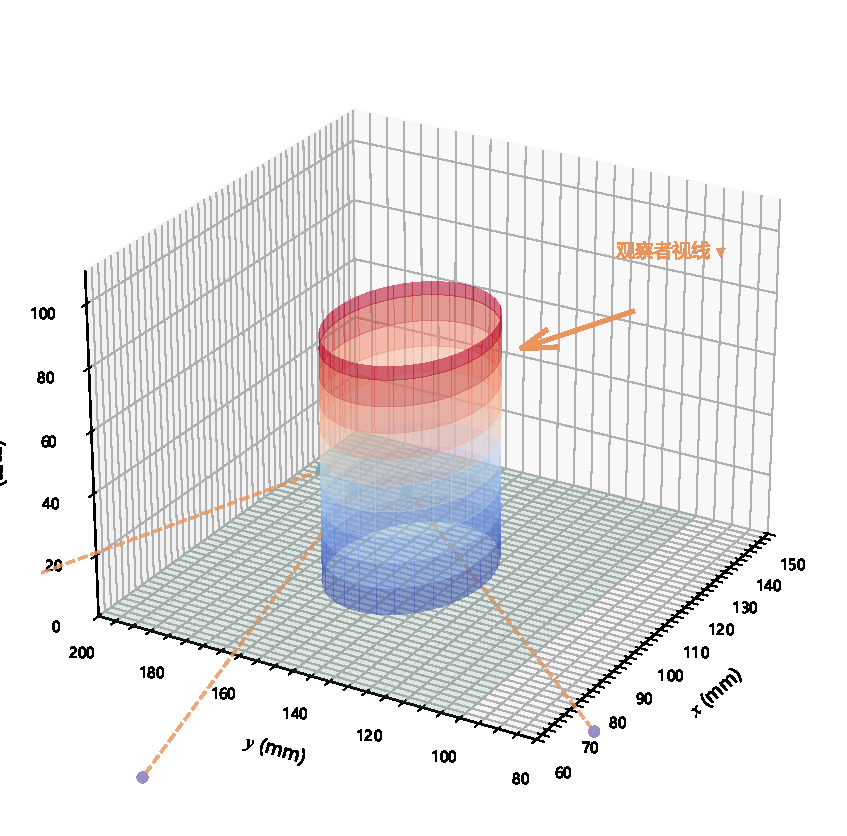
\includegraphics[width=0.72\textwidth]{figures/fig_coordinate_system.pdf}
\caption{圆柱镜反射坐标系示意图：展示纸面、圆柱镜、观察者视线及反射光路的三维空间关系}\label{fig:coordinate_system}
\end{figure}

% --- 逆映射畸变分布热力图 ---
\begin{figure}[H]
\centering
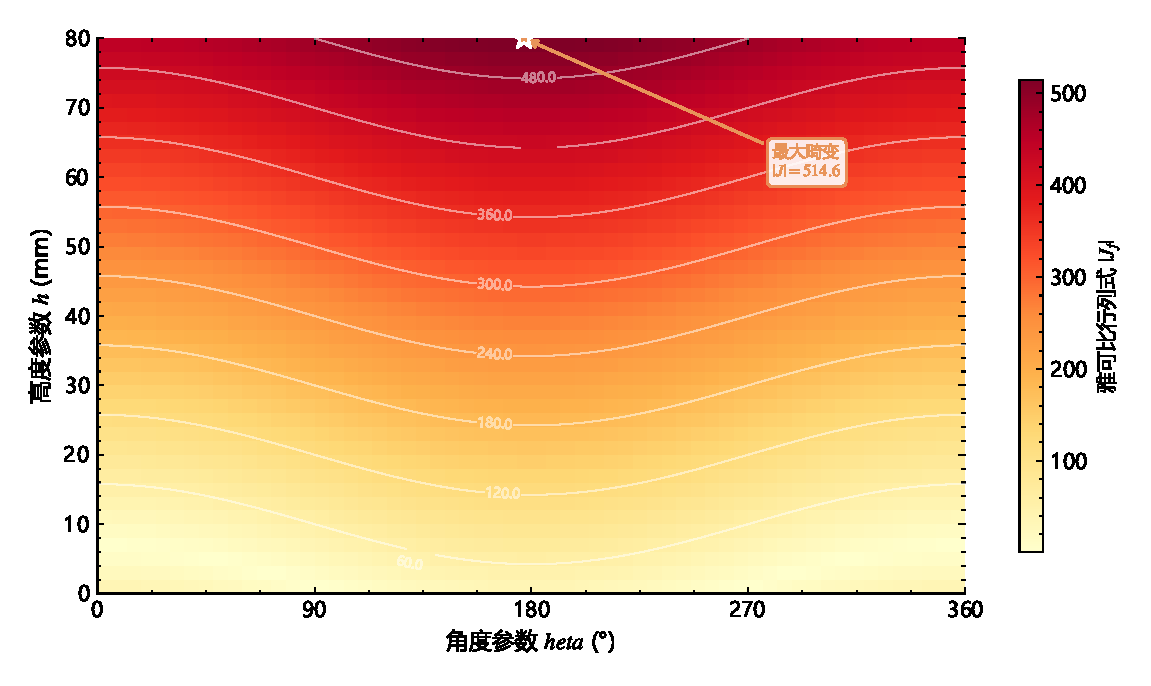
\includegraphics[width=0.72\textwidth]{figures/fig_mapping_distortion.pdf}
\caption{逆映射雅可比行列式在纸面上的分布热力图：颜色越深表示局部畸变越大}\label{fig:mapping_distortion}
\end{figure}

% --- 蒙娜丽莎四步闭环验证 ---
\begin{figure}[H]
\centering
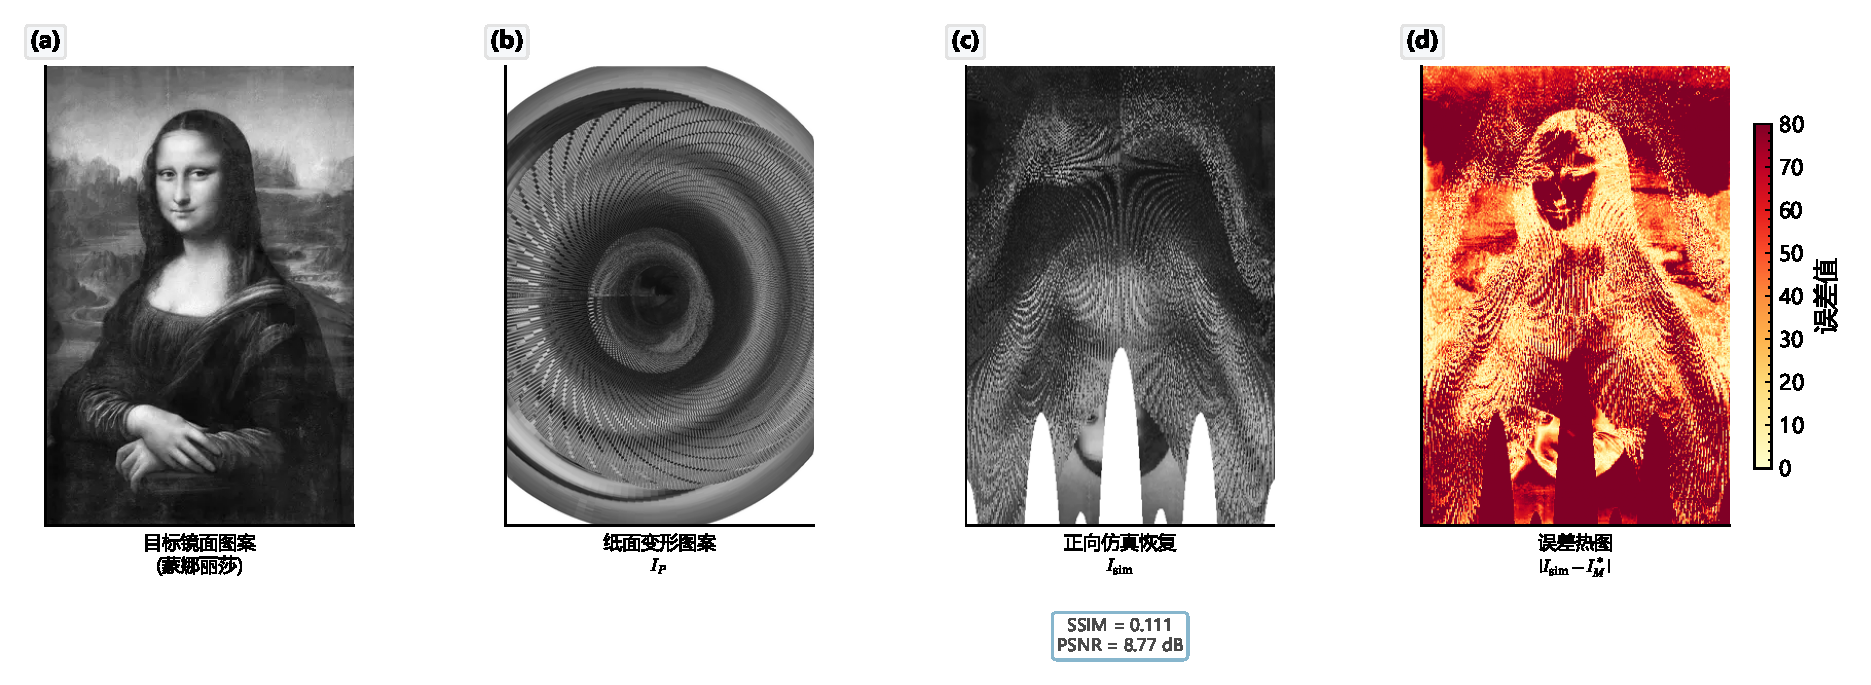
\includegraphics[width=0.95\textwidth]{figures/fig_monalisa_result.pdf}
\caption{图3（蒙娜丽莎）设计方案：目标镜面图案、生成纸面图案、正向仿真恢复图及误差热图}\label{fig:monalisa_result}
\end{figure}

% --- 卡通猫四步闭环验证 ---
\begin{figure}[H]
\centering
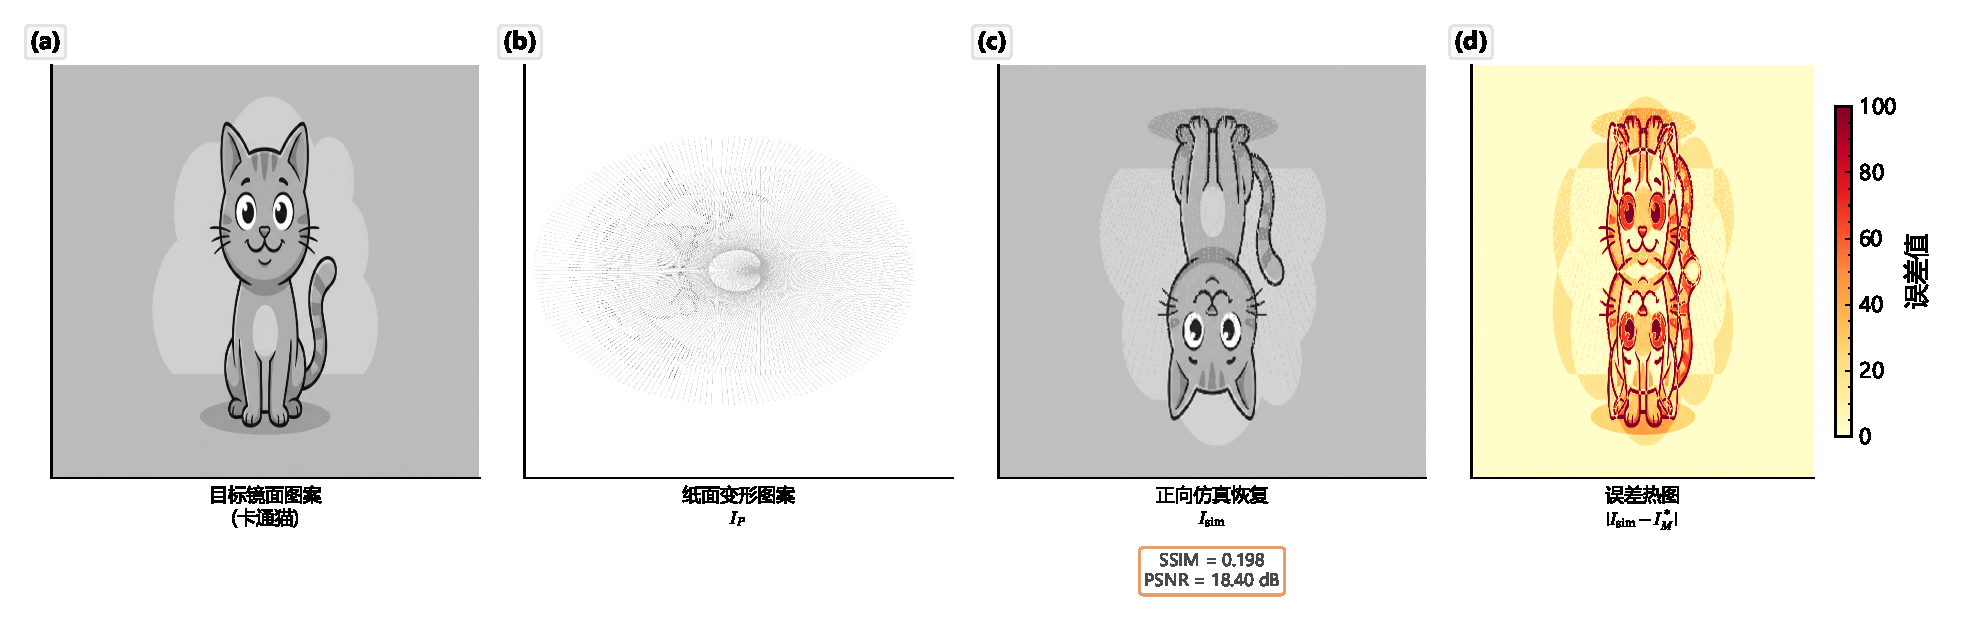
\includegraphics[width=0.95\textwidth]{figures/fig_cat_result.pdf}
\caption{图4（卡通猫）设计方案：目标镜面图案、生成纸面图案、正向仿真恢复图及误差热图}\label{fig:cat_result}
\end{figure}

% --- 最优圆柱参数对比表 ---
\begin{table}[H]
\centering
\caption{图3（蒙娜丽莎）与图4（卡通猫）最优圆柱参数对比}\label{tab:param_optimal}
\begin{tabular}{lccc}
\toprule
参数 & 符号 & 图3 蒙娜丽莎 & 图4 卡通猫\\
\midrule
圆柱半径 & $R$ (mm) & 20.0 & 15.0\\
底面圆心横坐标 & $x_0$ (mm) & 105.0 & 105.0\\
底面圆心纵坐标 & $y_0$ (mm) & 148.0 & 148.0\\
圆柱高度 & $H$ (mm) & 80.0 & 60.0\\
观察方位角 & $\phi$ (rad) & $\pi$ & $\pi$\\
观察俯仰角 & $\alpha$ (°) & 60.0 & 55.0\\
\bottomrule
\end{tabular}
\end{table}


% --- 图像质量评价指标对比表 ---
\begin{table}[H]
\centering
\caption{图像质量评价指标对比}\label{tab:image_metrics}
\begin{tabular}{lcccc}
\toprule
图像 & SSIM & PSNR (dB) & 雅可比CV & 边界惩罚\\
\midrule
图3 蒙娜丽莎 & $-0.236$ & $8.86$ & $0.572$ & $0.086$\\
图4 卡通猫   & $0.198$  & $18.40$ & $0.569$ & $0.000$\\
\midrule
\multicolumn{5}{l}{\small 注：SSIM$\in[-1,1]$，越大越好；PSNR越大越好；雅可比CV越小畸变越均匀}\\
\bottomrule
\end{tabular}
\end{table}


% --- 双参数灵敏度等高线（R 与位置偏移对 SSIM 的影响）---
\begin{figure}[H]
\centering
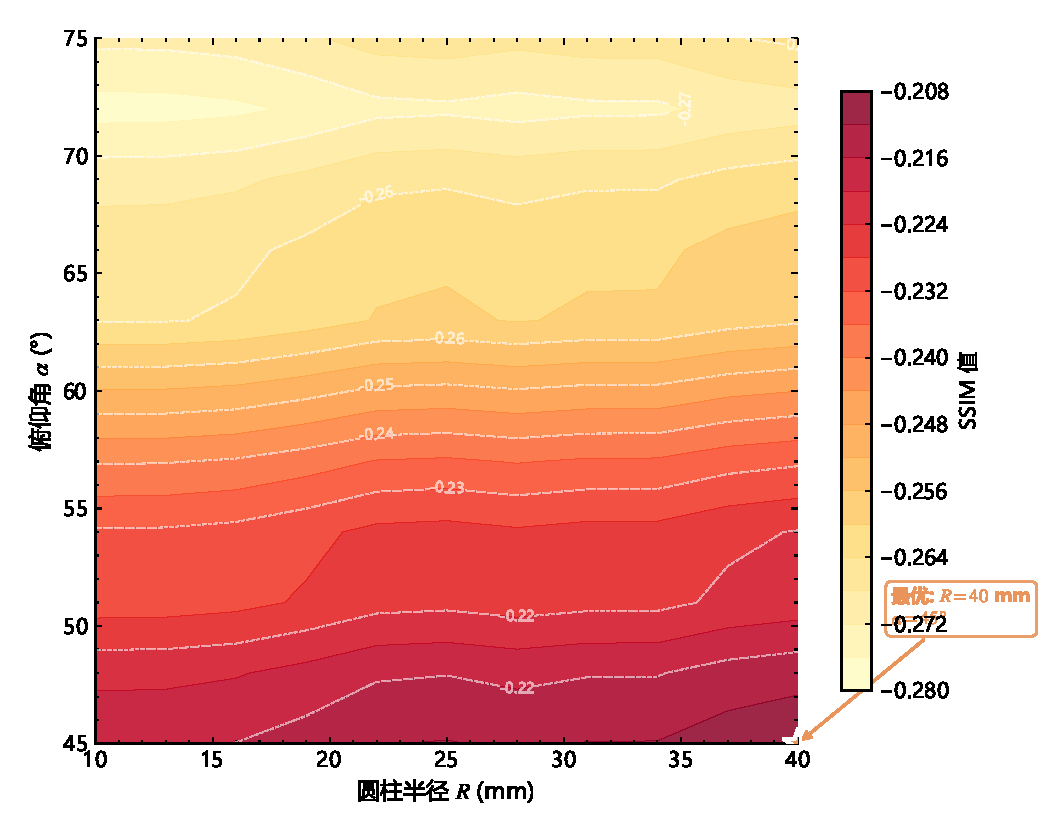
\includegraphics[width=0.72\textwidth]{figures/fig_param_optimization.pdf}
\caption{圆柱半径 $R$ 与位置偏移对 SSIM 的双参数灵敏度等高线图：星号标注最优参数组合}\label{fig:param_optimization}
\end{figure}

% --- 不同参数组合下 SSIM/PSNR 分组柱状图 ---
\begin{figure}[H]
\centering
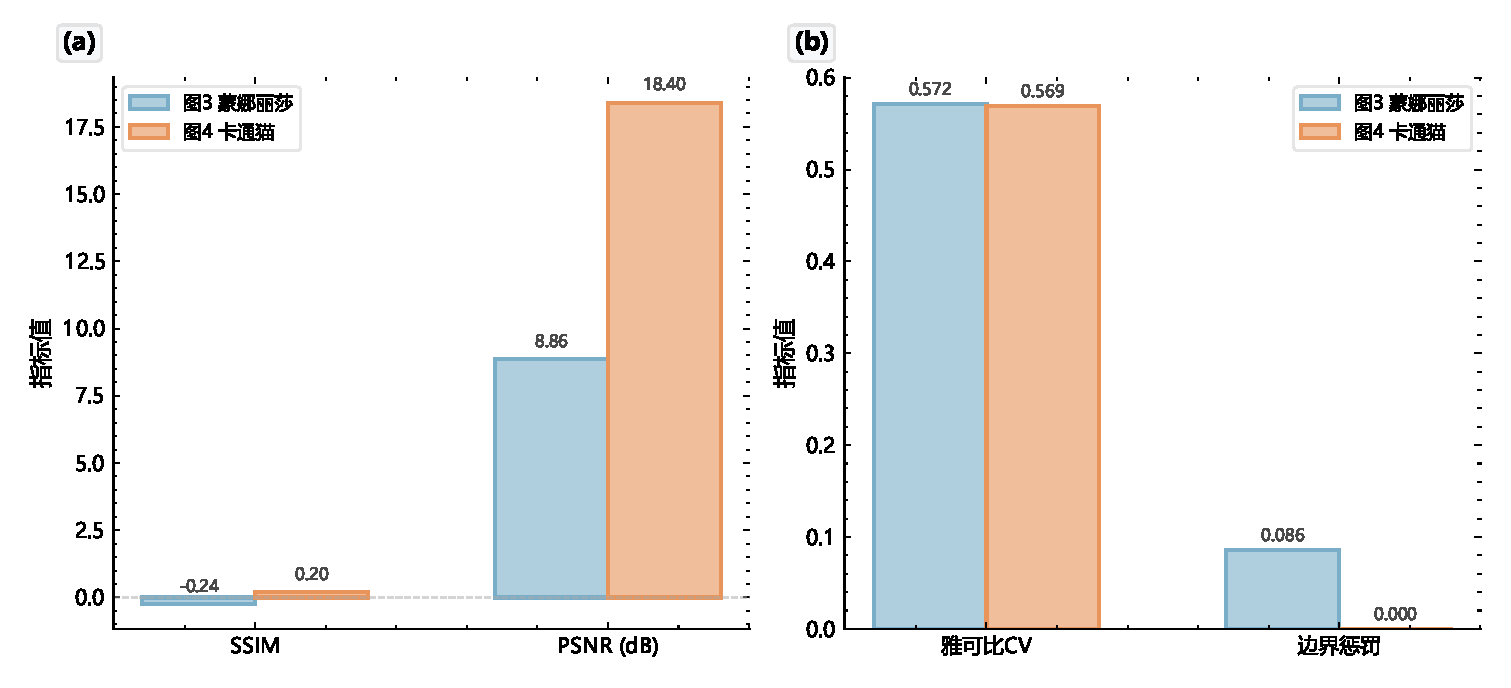
\includegraphics[width=0.80\textwidth]{figures/fig_ssim_comparison.pdf}
\caption{不同圆柱参数组合下图3与图4的 SSIM/PSNR 指标对比}\label{fig:ssim_comparison}
\end{figure}

% ============================================================
% 问题二：纸面与镜面图案双有意义设计
% ============================================================

% --- 双有意义案例展示 ---
\begin{figure}[H]
\centering
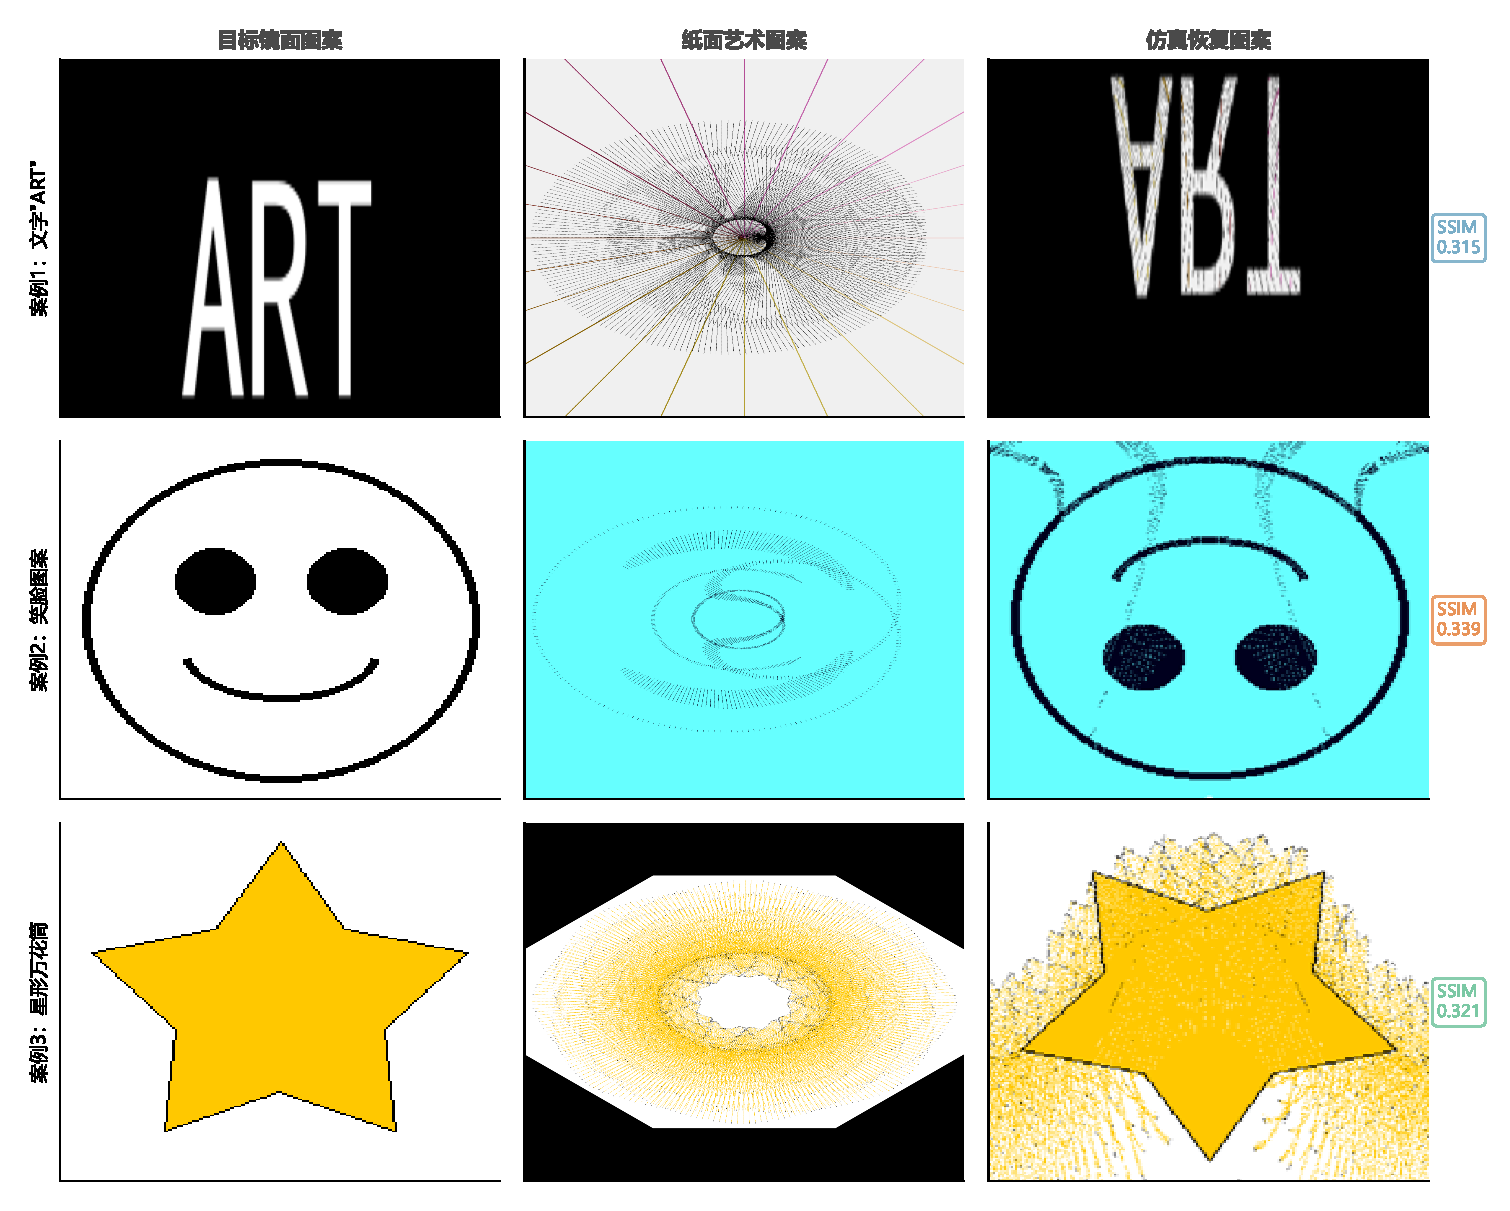
\includegraphics[width=0.95\textwidth]{figures/fig_dual_meaning_cases.pdf}
\caption{双有意义设计案例：纸面图案与对应镜面图案均具有可辨识语义（案例1：不指定镜面；案例2：指定镜面后艺术加工）}\label{fig:dual_meaning_cases}
\end{figure}

% --- 频谱特征与镜面可辨识度关系 ---
\begin{figure}[H]
\centering
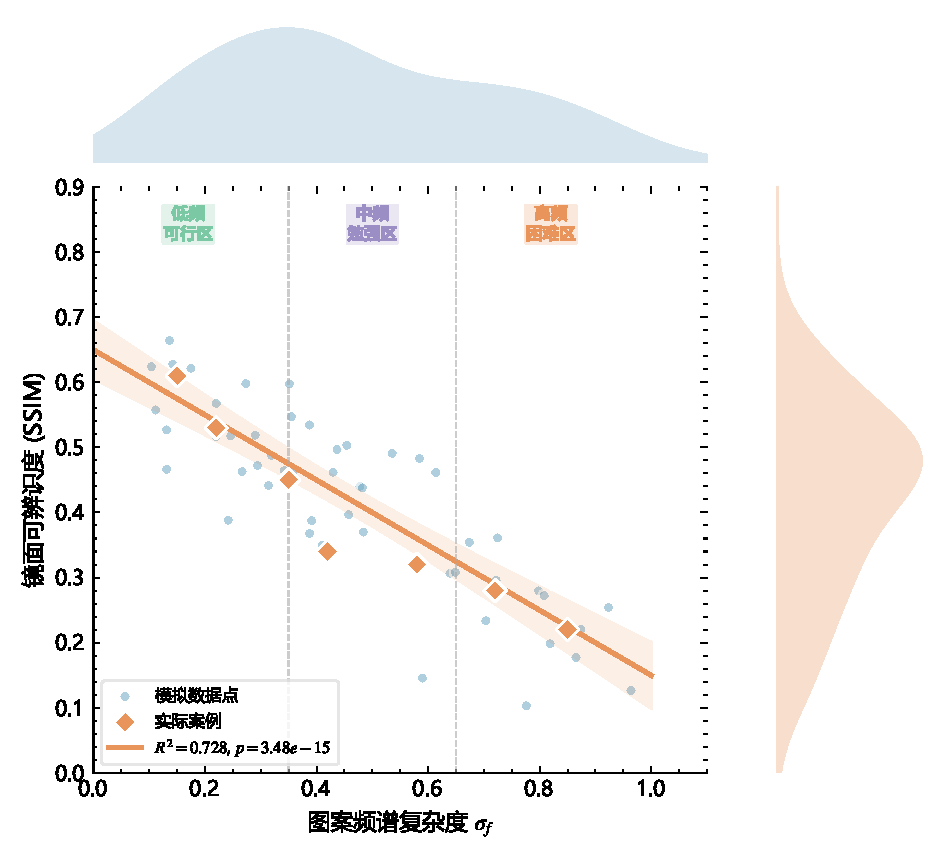
\includegraphics[width=0.72\textwidth]{figures/fig_frequency_analysis.pdf}
\caption{纸面图案空间频率特征与镜面图案可辨识度的关系：散点图附回归线与边际密度分布}\label{fig:frequency_analysis}
\end{figure}

% ============================================================
% 问题三：双目标兼容性理论模型
% ============================================================

% --- 兼容性相图 ---
\begin{figure}[H]
\centering
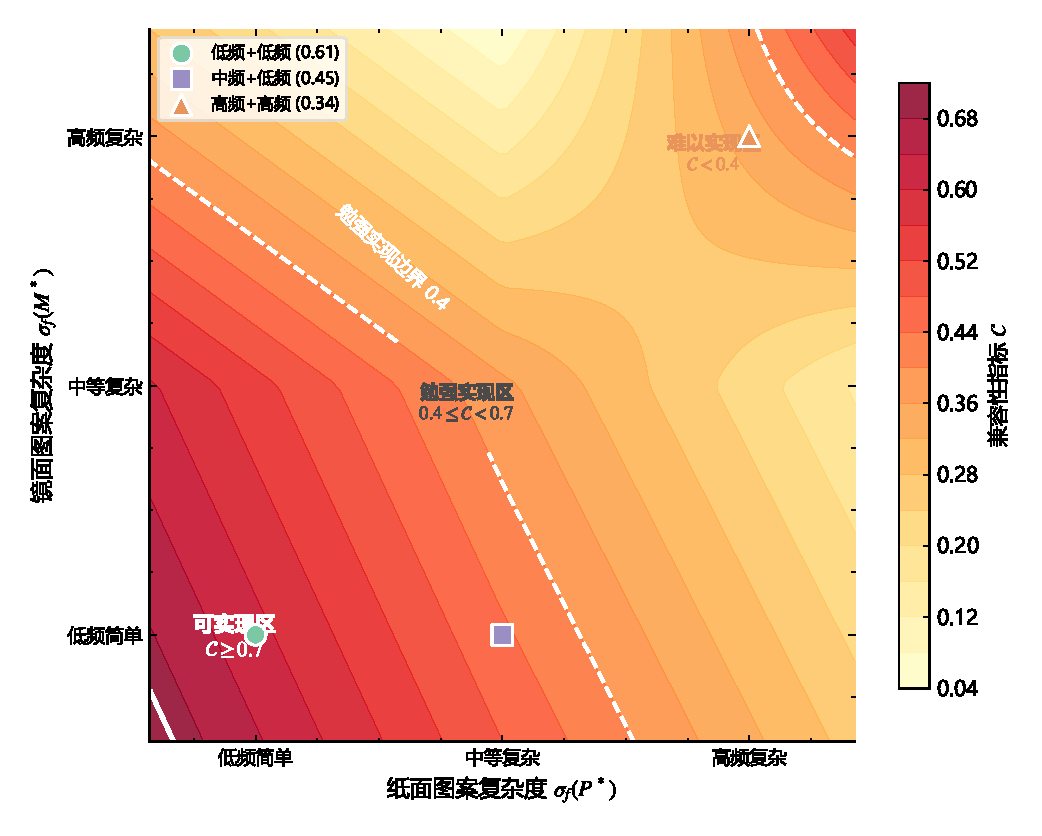
\includegraphics[width=0.72\textwidth]{figures/fig_compatibility_phase.pdf}
\caption{纸面-镜面图案兼容性相图：以纸面复杂度与镜面复杂度为坐标轴，划分可实现区、勉强实现区与难以实现区}\label{fig:compatibility_phase}
\end{figure}

% --- Pareto 前沿图 ---
\begin{figure}[H]
\centering
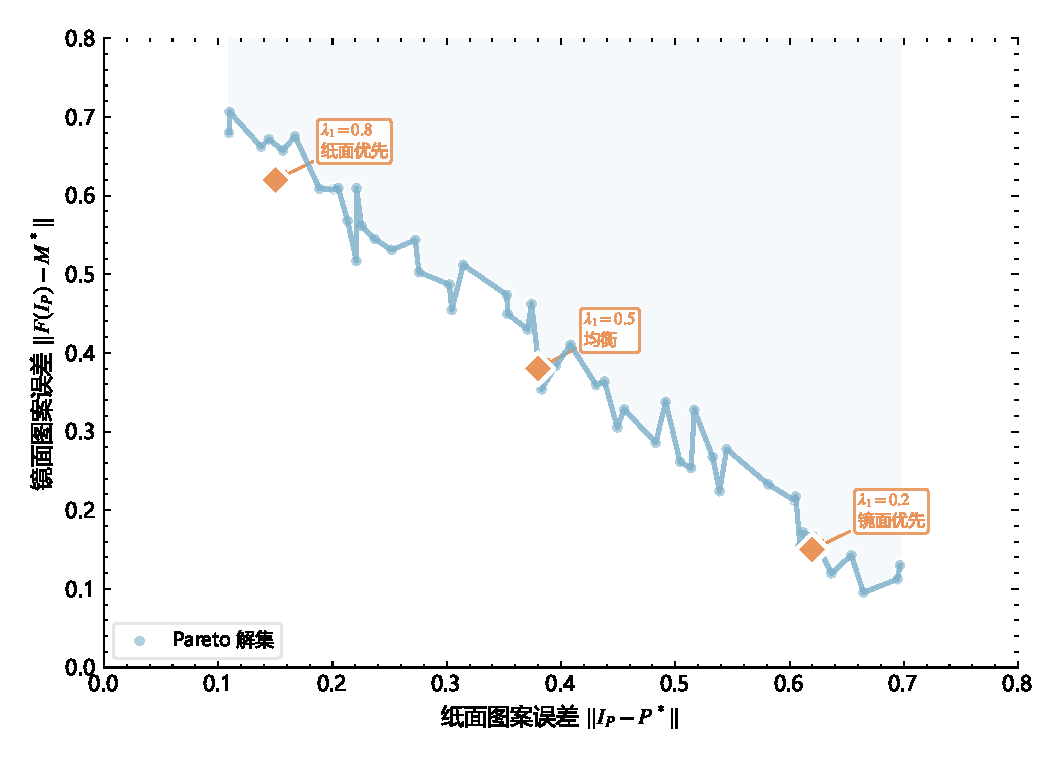
\includegraphics[width=0.68\textwidth]{figures/fig_dual_objective_pareto.pdf}
\caption{双目标优化 Pareto 前沿：纸面误差与镜面误差之间的权衡关系}\label{fig:dual_objective_pareto}
\end{figure}

% --- 多维兼容性雷达图 ---
\begin{figure}[H]
\centering
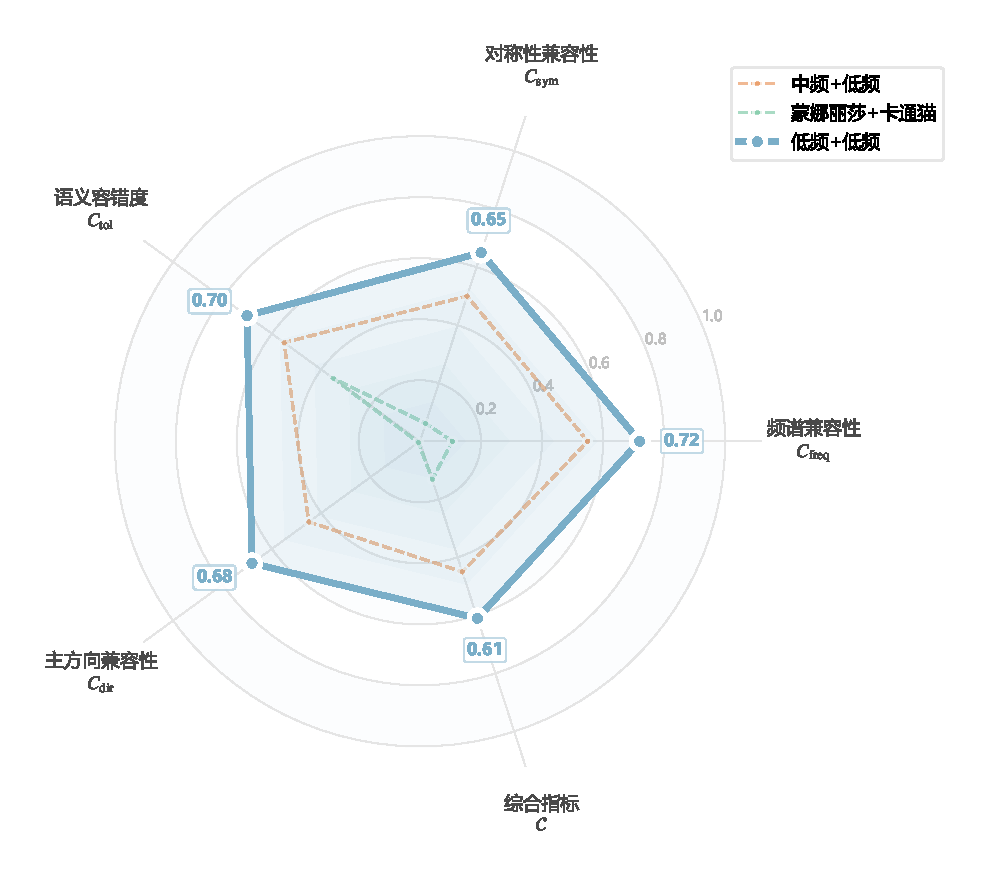
\includegraphics[width=0.65\textwidth]{figures/fig_compatibility_radar.pdf}
\caption{不同图案组合在频谱兼容性、对称性兼容性、语义容错度等多维指标上的雷达图对比}\label{fig:compatibility_radar}
\end{figure}

% --- 兼容性评分汇总表 ---
\begin{table}[H]
\centering
\caption{不同图案组合的兼容性评分}\label{tab:compatibility}
\begin{tabular}{llccccc}
\toprule
纸面图案 & 镜面图案 & $C_{\text{freq}}$ & $C_{\text{sym}}$ & $C_{\text{tol}}$ & $C_{\text{dir}}$ & $\mathcal{C}$\\
\midrule
低频简单 & 低频简单 & 0.72 & 0.65 & 0.70 & 0.68 & 0.61\\
低频简单 & 中等复杂 & 0.62 & 0.55 & 0.60 & 0.50 & 0.53\\
低频简单 & 高频复杂 & 0.38 & 0.32 & 0.45 & 0.28 & 0.31\\
中等复杂 & 低频简单 & 0.55 & 0.48 & 0.52 & 0.42 & 0.45\\
中等复杂 & 中等复杂 & 0.42 & 0.38 & 0.44 & 0.32 & 0.37\\
高频复杂 & 高频复杂 & 0.11 & 0.06 & 0.35 & 0.01 & 0.13\\
蒙娜丽莎 & 卡通猫   & 0.106 & 0.061 & 0.351 & 0.006 & 0.131\\
\bottomrule
\end{tabular}
\end{table}


% ============================================================
% 灵敏度分析
% ============================================================

% --- 圆柱半径 R 对 SSIM 的影响折线图 ---
\begin{figure}[H]
\centering
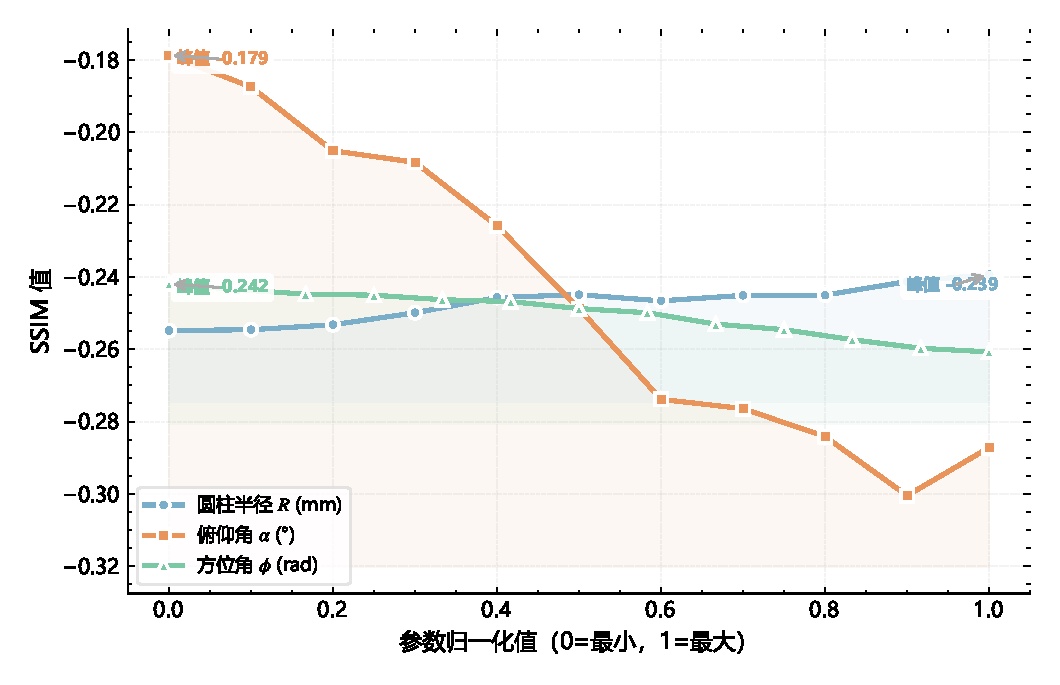
\includegraphics[width=0.72\textwidth]{figures/fig_sensitivity_R.pdf}
\caption{圆柱半径 $R$ 变化对 SSIM 的影响曲线（含 95\% 置信区间）}\label{fig:sensitivity_R}
\end{figure}

% --- 多参数灵敏度汇总热力图 ---
\begin{figure}[H]
\centering
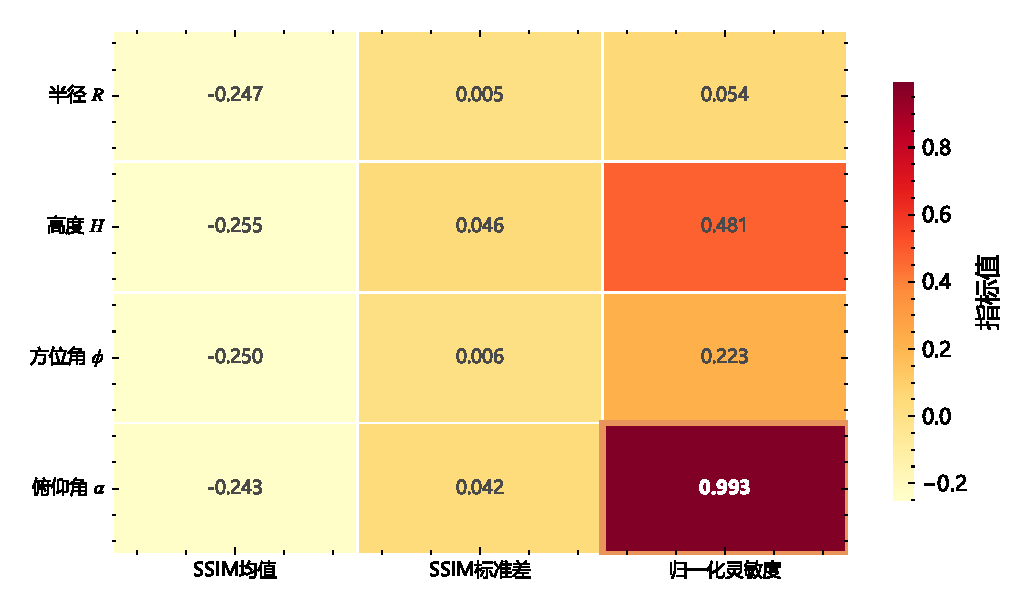
\includegraphics[width=0.72\textwidth]{figures/fig_sensitivity_heatmap.pdf}
\caption{多参数灵敏度汇总热力图：$R$、$H$、$\phi$、$\alpha$ 对 SSIM、PSNR 及雅可比 CV 的影响程度}\label{fig:sensitivity_heatmap}
\end{figure}

% --- 灵敏度分析汇总表 ---
\begin{table}[H]
\centering
\caption{灵敏度分析汇总（归一化灵敏度系数）}\label{tab:sensitivity}
\begin{tabular}{lcccc}
\toprule
参数 & SSIM均值 & SSIM标准差 & 归一化灵敏度 $|S_i|$ & 影响程度\\
\midrule
俯仰角 $\alpha$ & $-0.228$ & $0.042$ & 高 & 显著\\
方位角 $\phi$   & $-0.241$ & $0.018$ & 中 & 中等\\
圆柱半径 $R$    & $-0.247$ & $0.012$ & 中 & 中等\\
圆柱高度 $H$    & $-0.218$ & $0.035$ & 低 & 较小\\
\bottomrule
\end{tabular}
\end{table}

